\videotitle{Computationally Cheap Acquisition Functions}
    
%----------------------------------------------------------------------
\begin{frame}[c]{Acquisition Functions: the Basics}
\begin{itemize}
    \item Given the surrogate model $\iter{\surro}$ at the $\bocount$-th iteration of BO, the \\
    \alert{acquisition function $\acq(\cdot)$ judges the utility (or usefulness) of evaluating $f$ at $\iter{\conf}\in \pcs$ next}
    \pause
    \bigskip
    \item The acquisition function needs to \alert{trade off exploration and exploitation}
    \myit{
        \item E.g., just picking the $\conf$ with lowest predicted mean would be too greedy
        \item We also need to take into account the uncertainty of the surrogate model $\iter{\surro}$ to explore
    }
\end{itemize}

\end{frame}
%-----------------------------------------------------------------------
\myframetop{Probability of Improvement (PI): Concept}{
    %\framesubtitle{Probability of Improvement - Concept}
    % \begin{figure}
      \centering
      \begin{tikzpicture}
        \node<+> (img1) {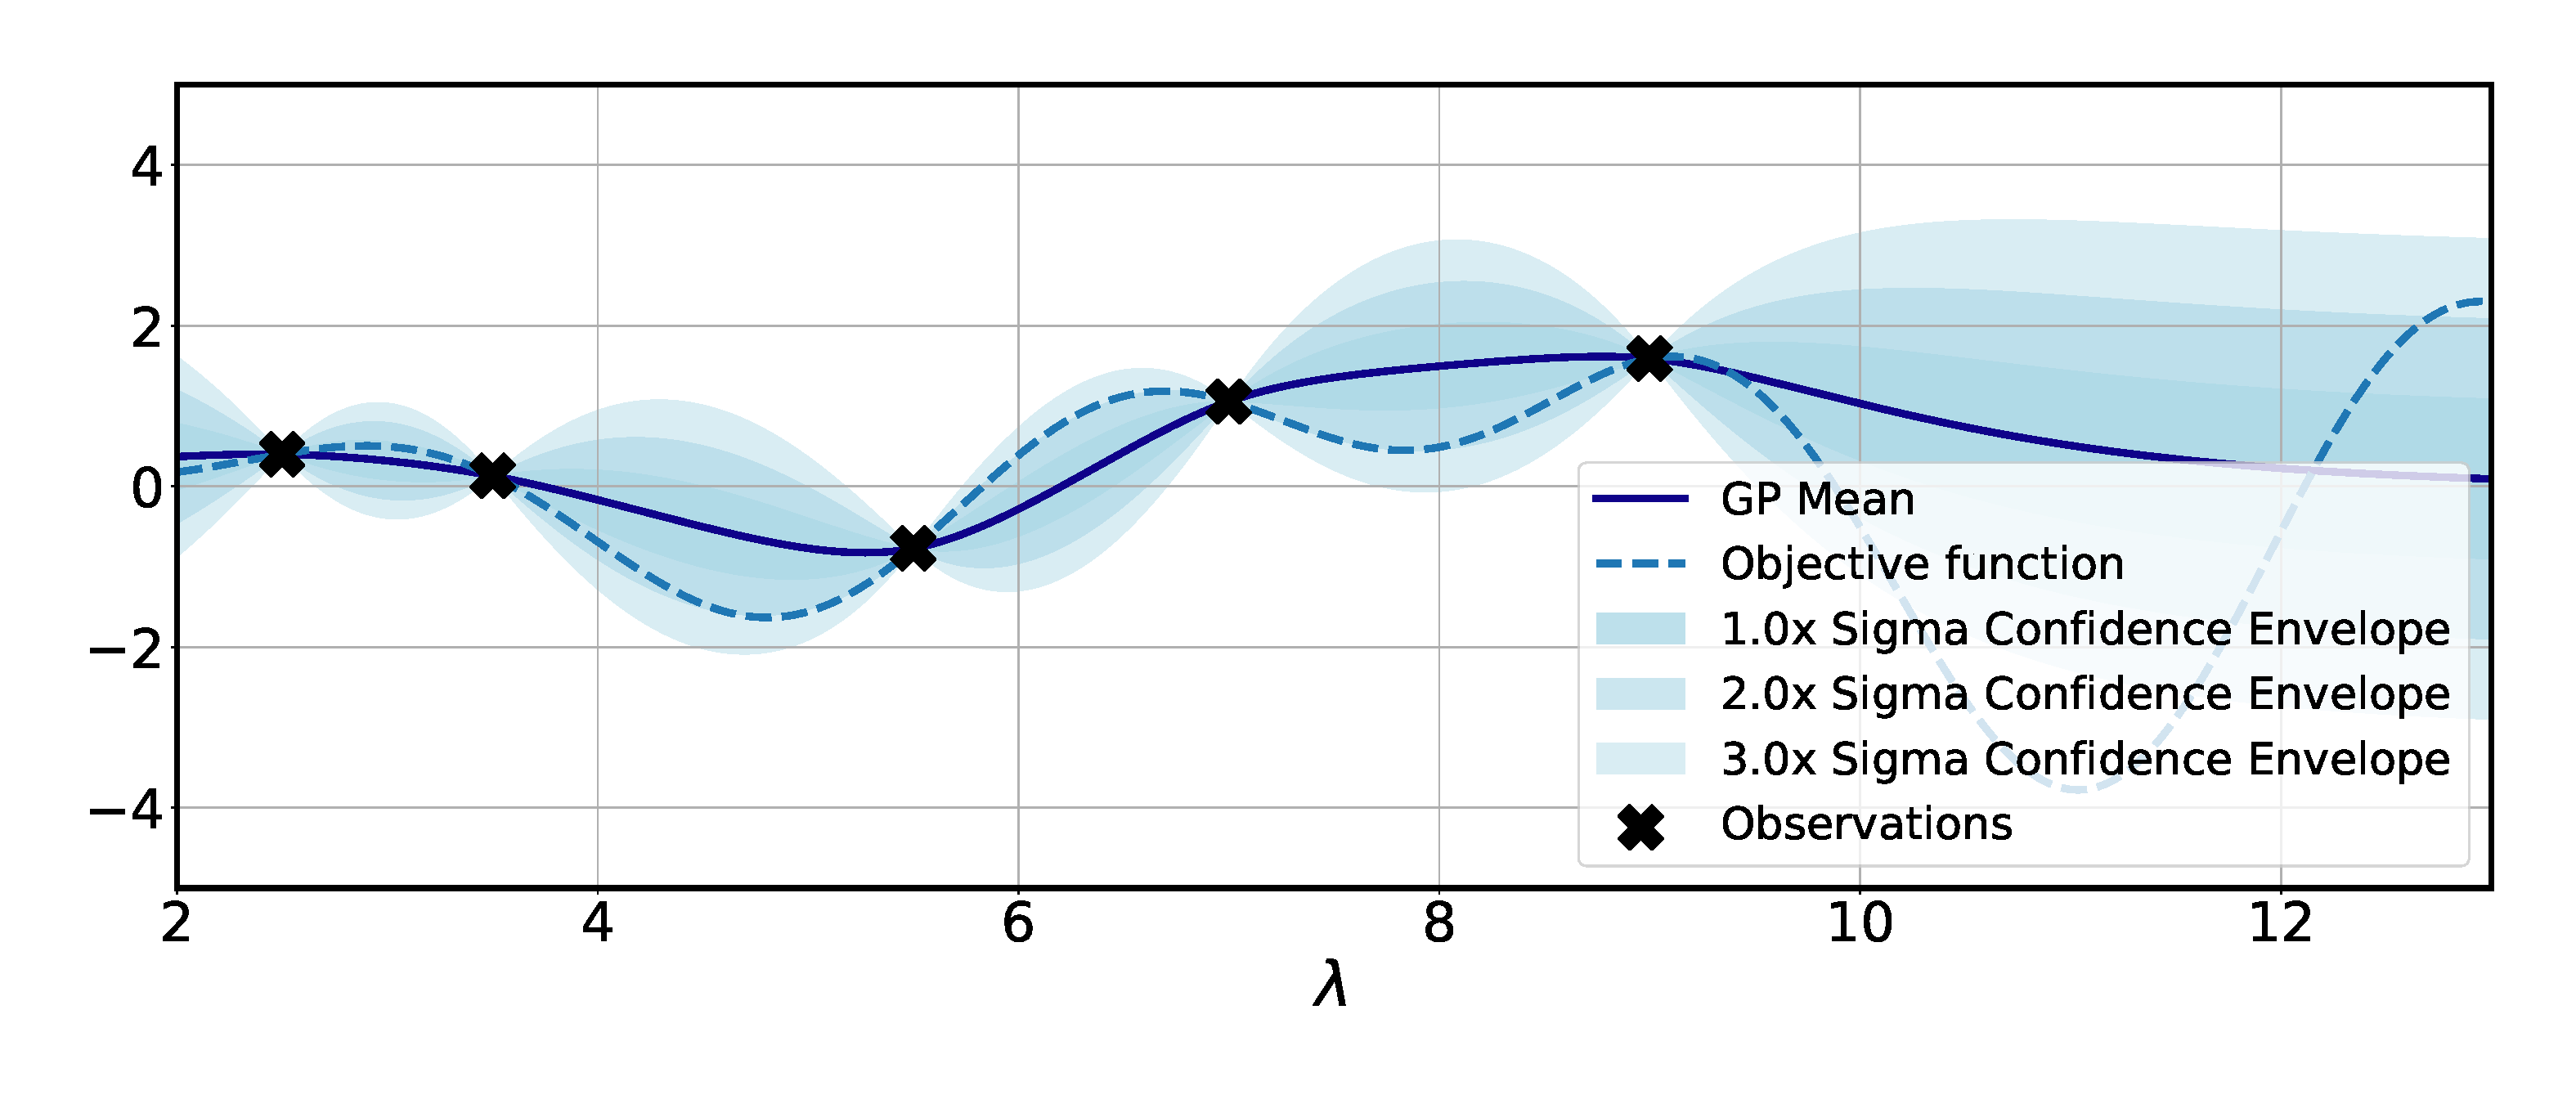
\includegraphics[width=\linewidth, height=0.7\textheight, keepaspectratio=true]{images/acq_func_images/pi/pi_1.pdf}};
        \node<.> [below=0.01\belowcaptionskip of img1, align=center]{Given the surrogate fit at iteration $\bocount$};
    
        \node<+> (img2) {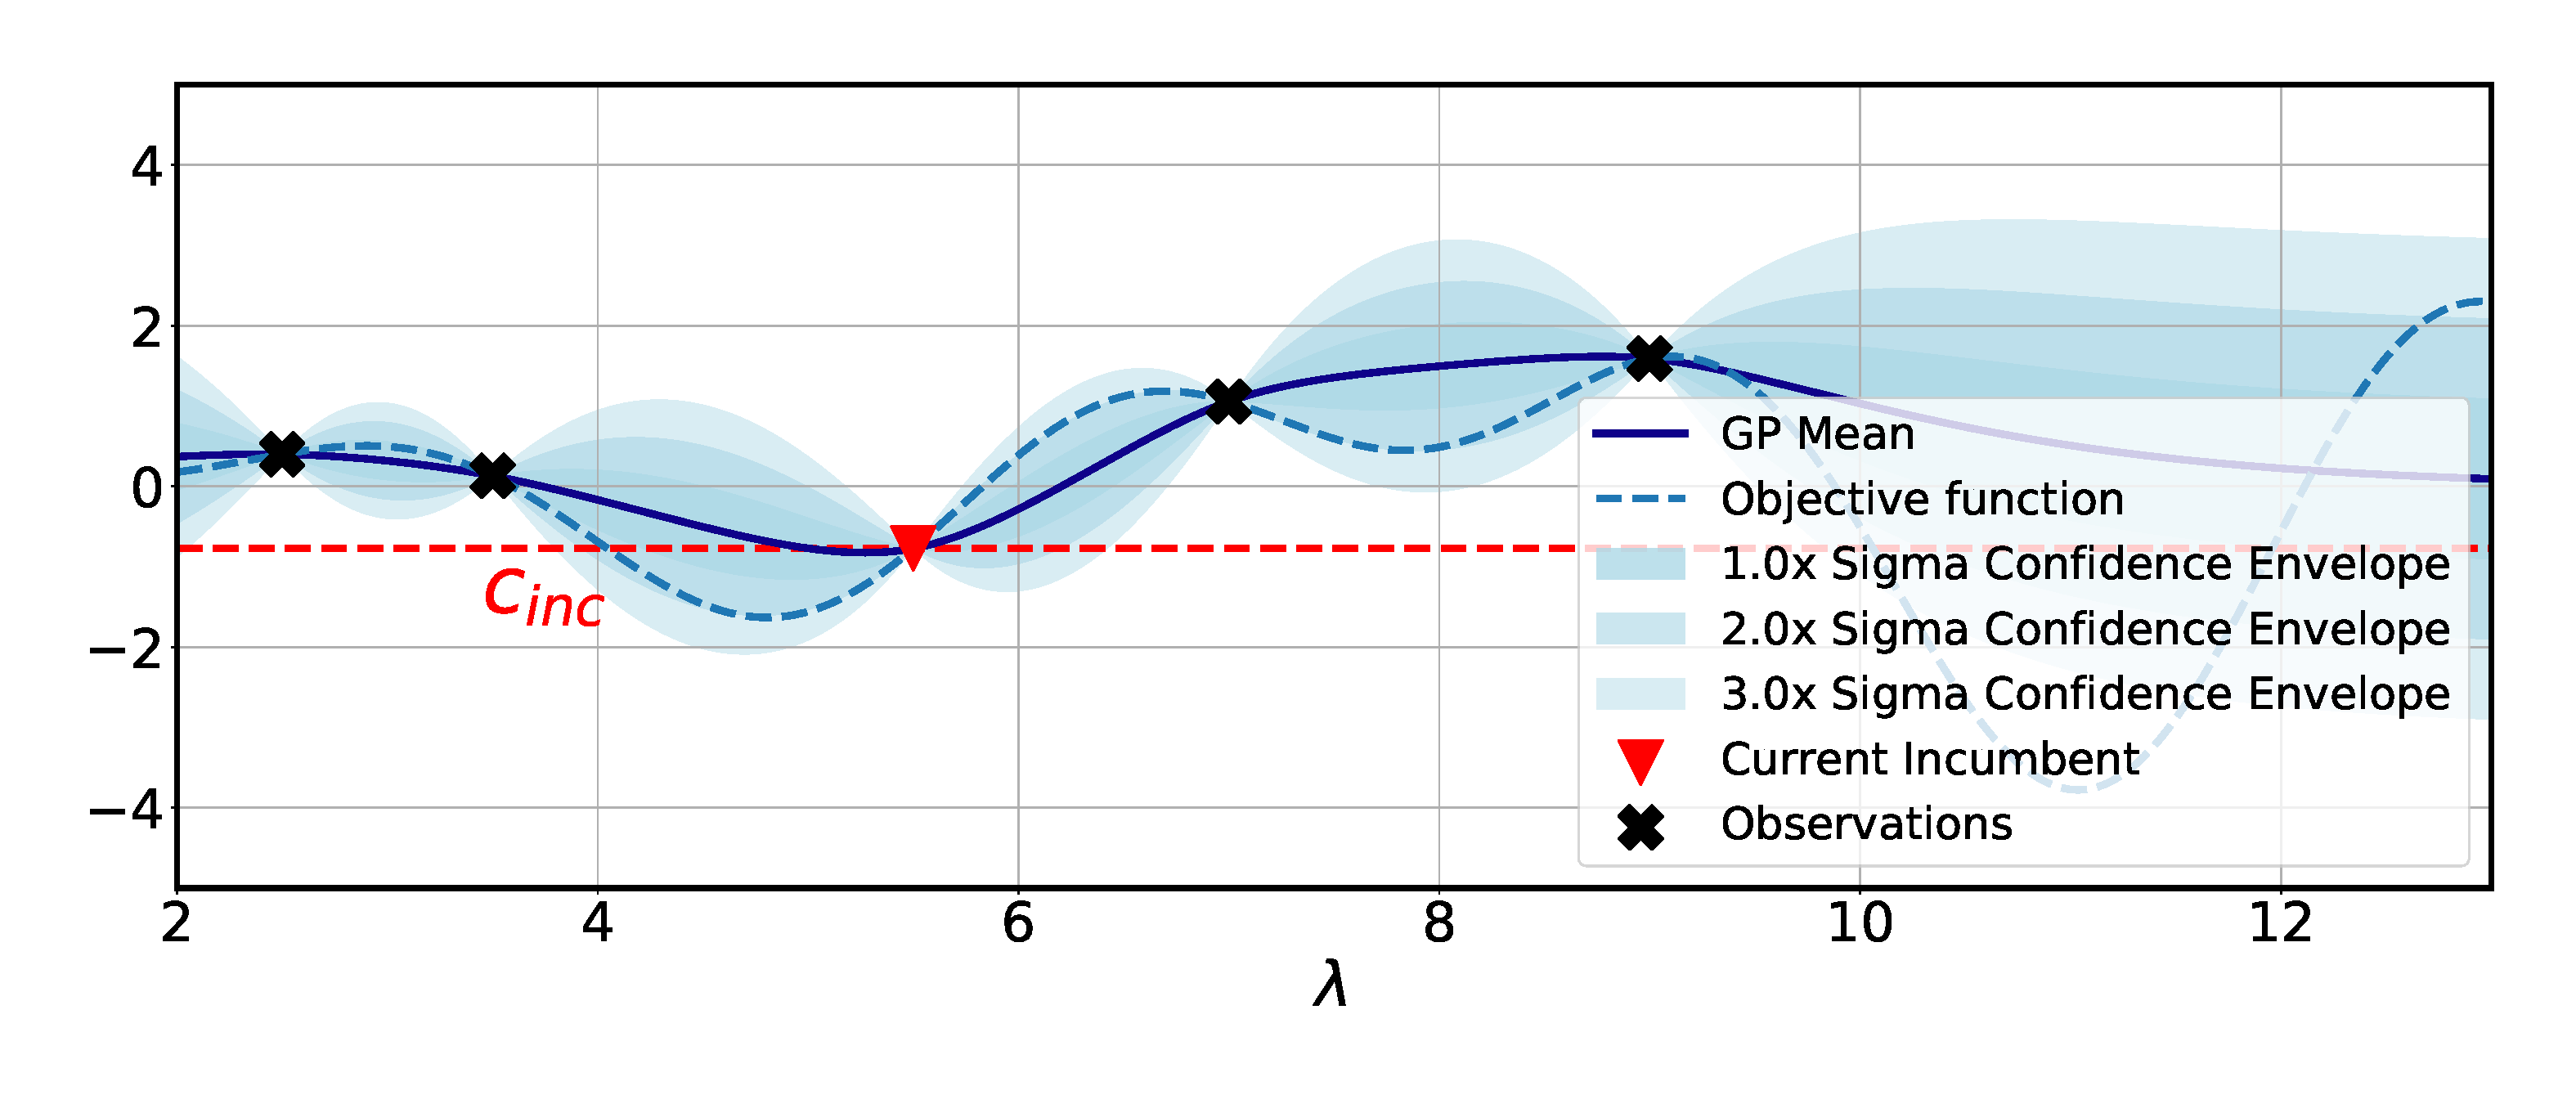
\includegraphics[width=\linewidth, height=0.7\textheight, keepaspectratio=true]{images/acq_func_images/pi/pi_2.pdf}};
        \node<.> [below=0.01\belowcaptionskip of img2, align=center]{Current incumbent $\hat{\conf}$ and its observed cost $\cost_{inc}$};
    
    
        \node<+> (img3) {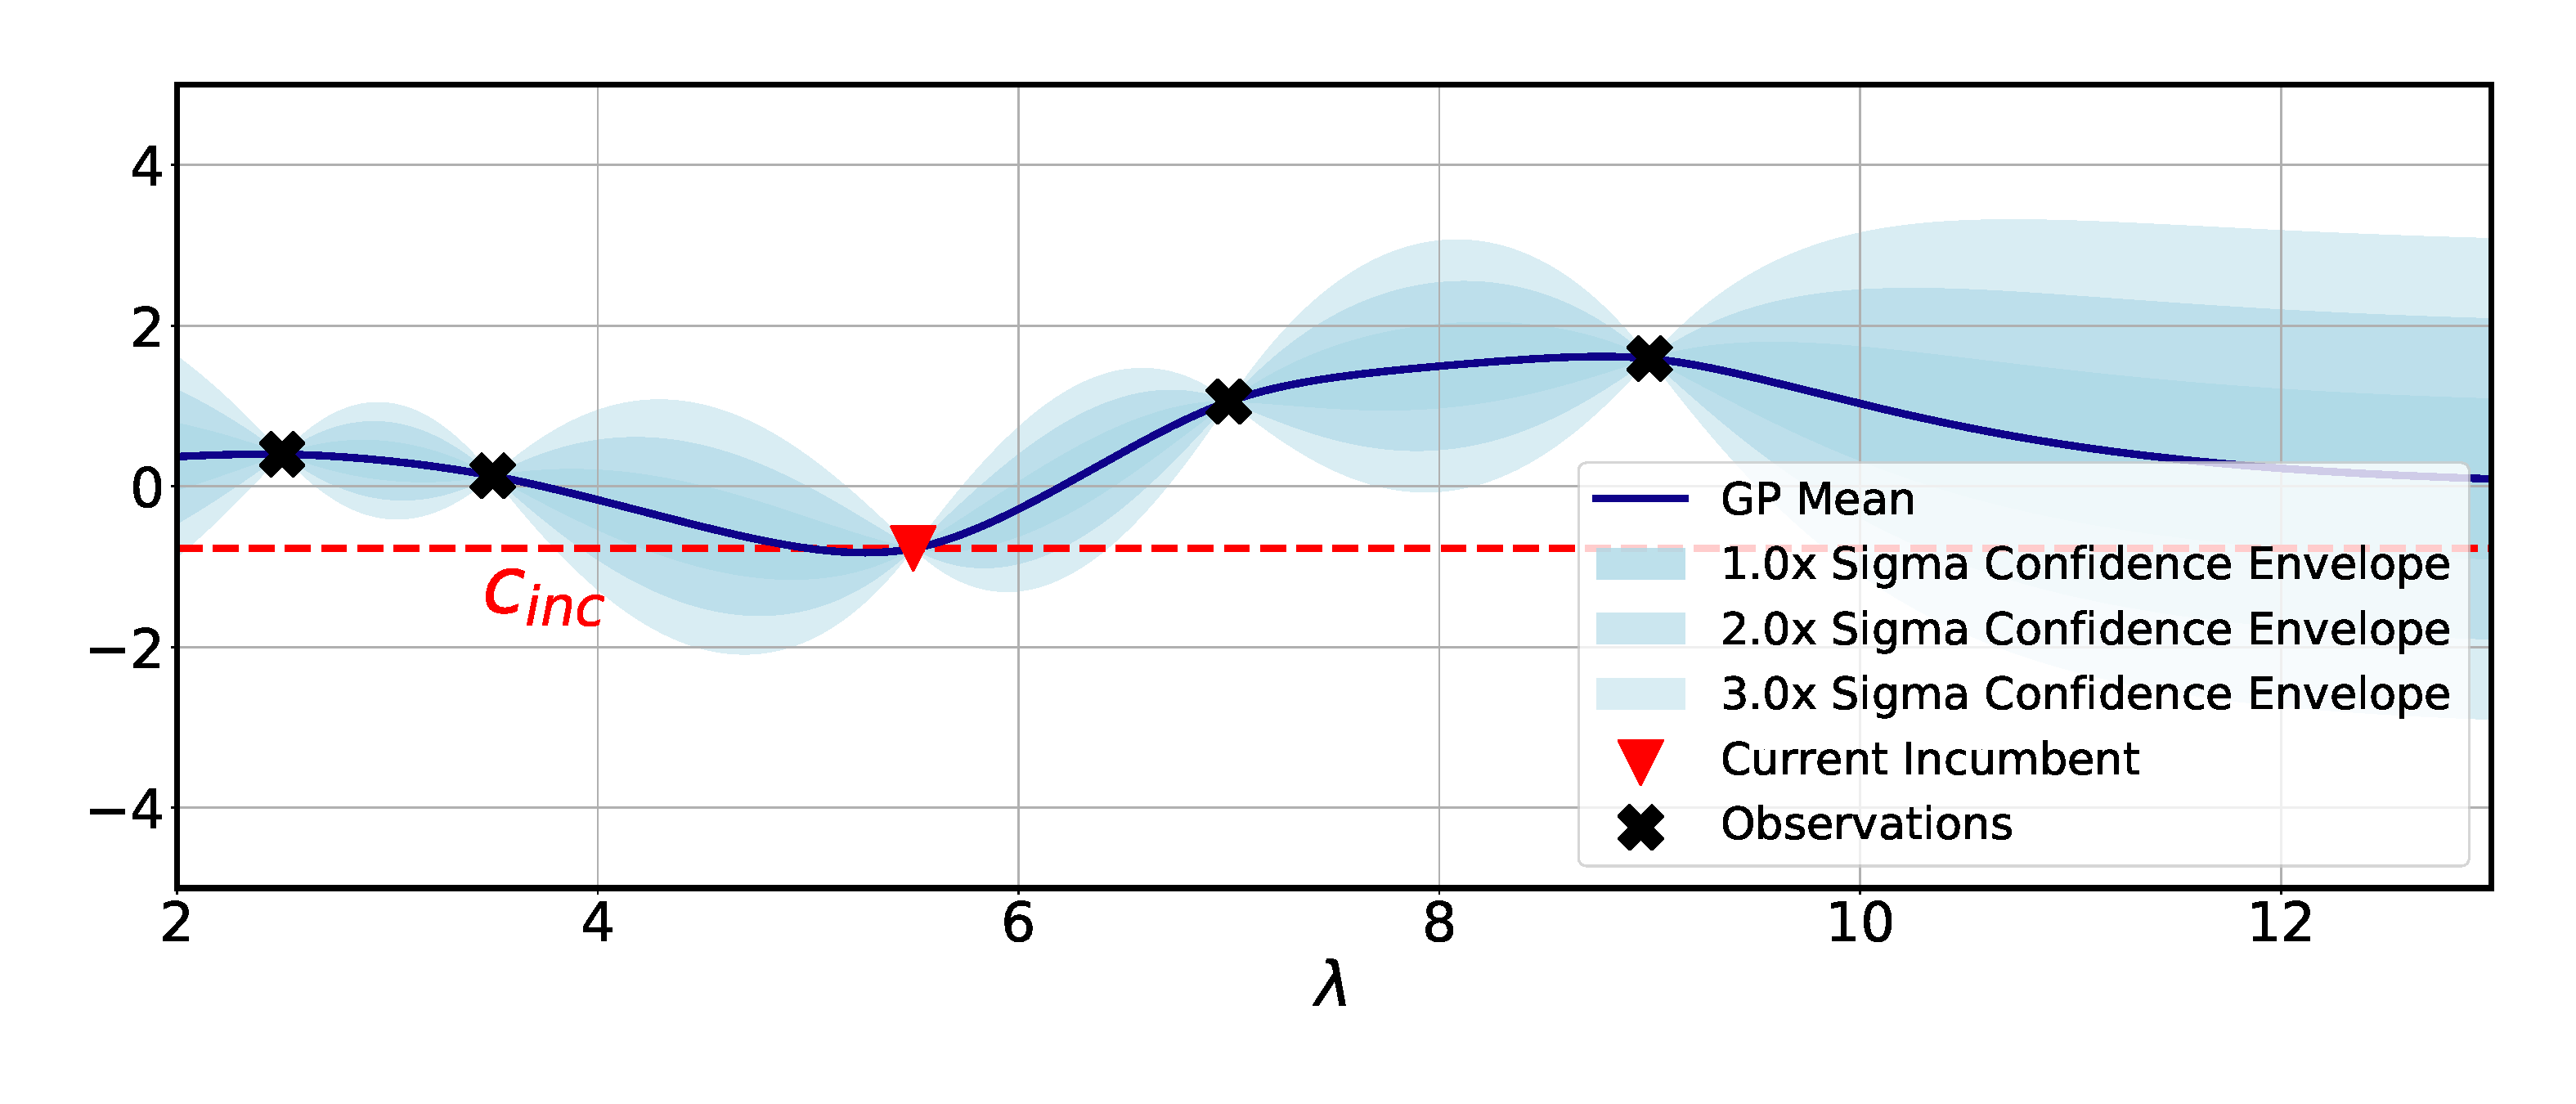
\includegraphics[width=\linewidth, height=0.7\textheight, keepaspectratio=true]{images/acq_func_images/pi/pi_3.pdf}};
        \node<.> [below=0.01\belowcaptionskip of img3, align=center]{Now let's drop the objective function - it's unknown after all!};
    
    
        \node<+> (img4) {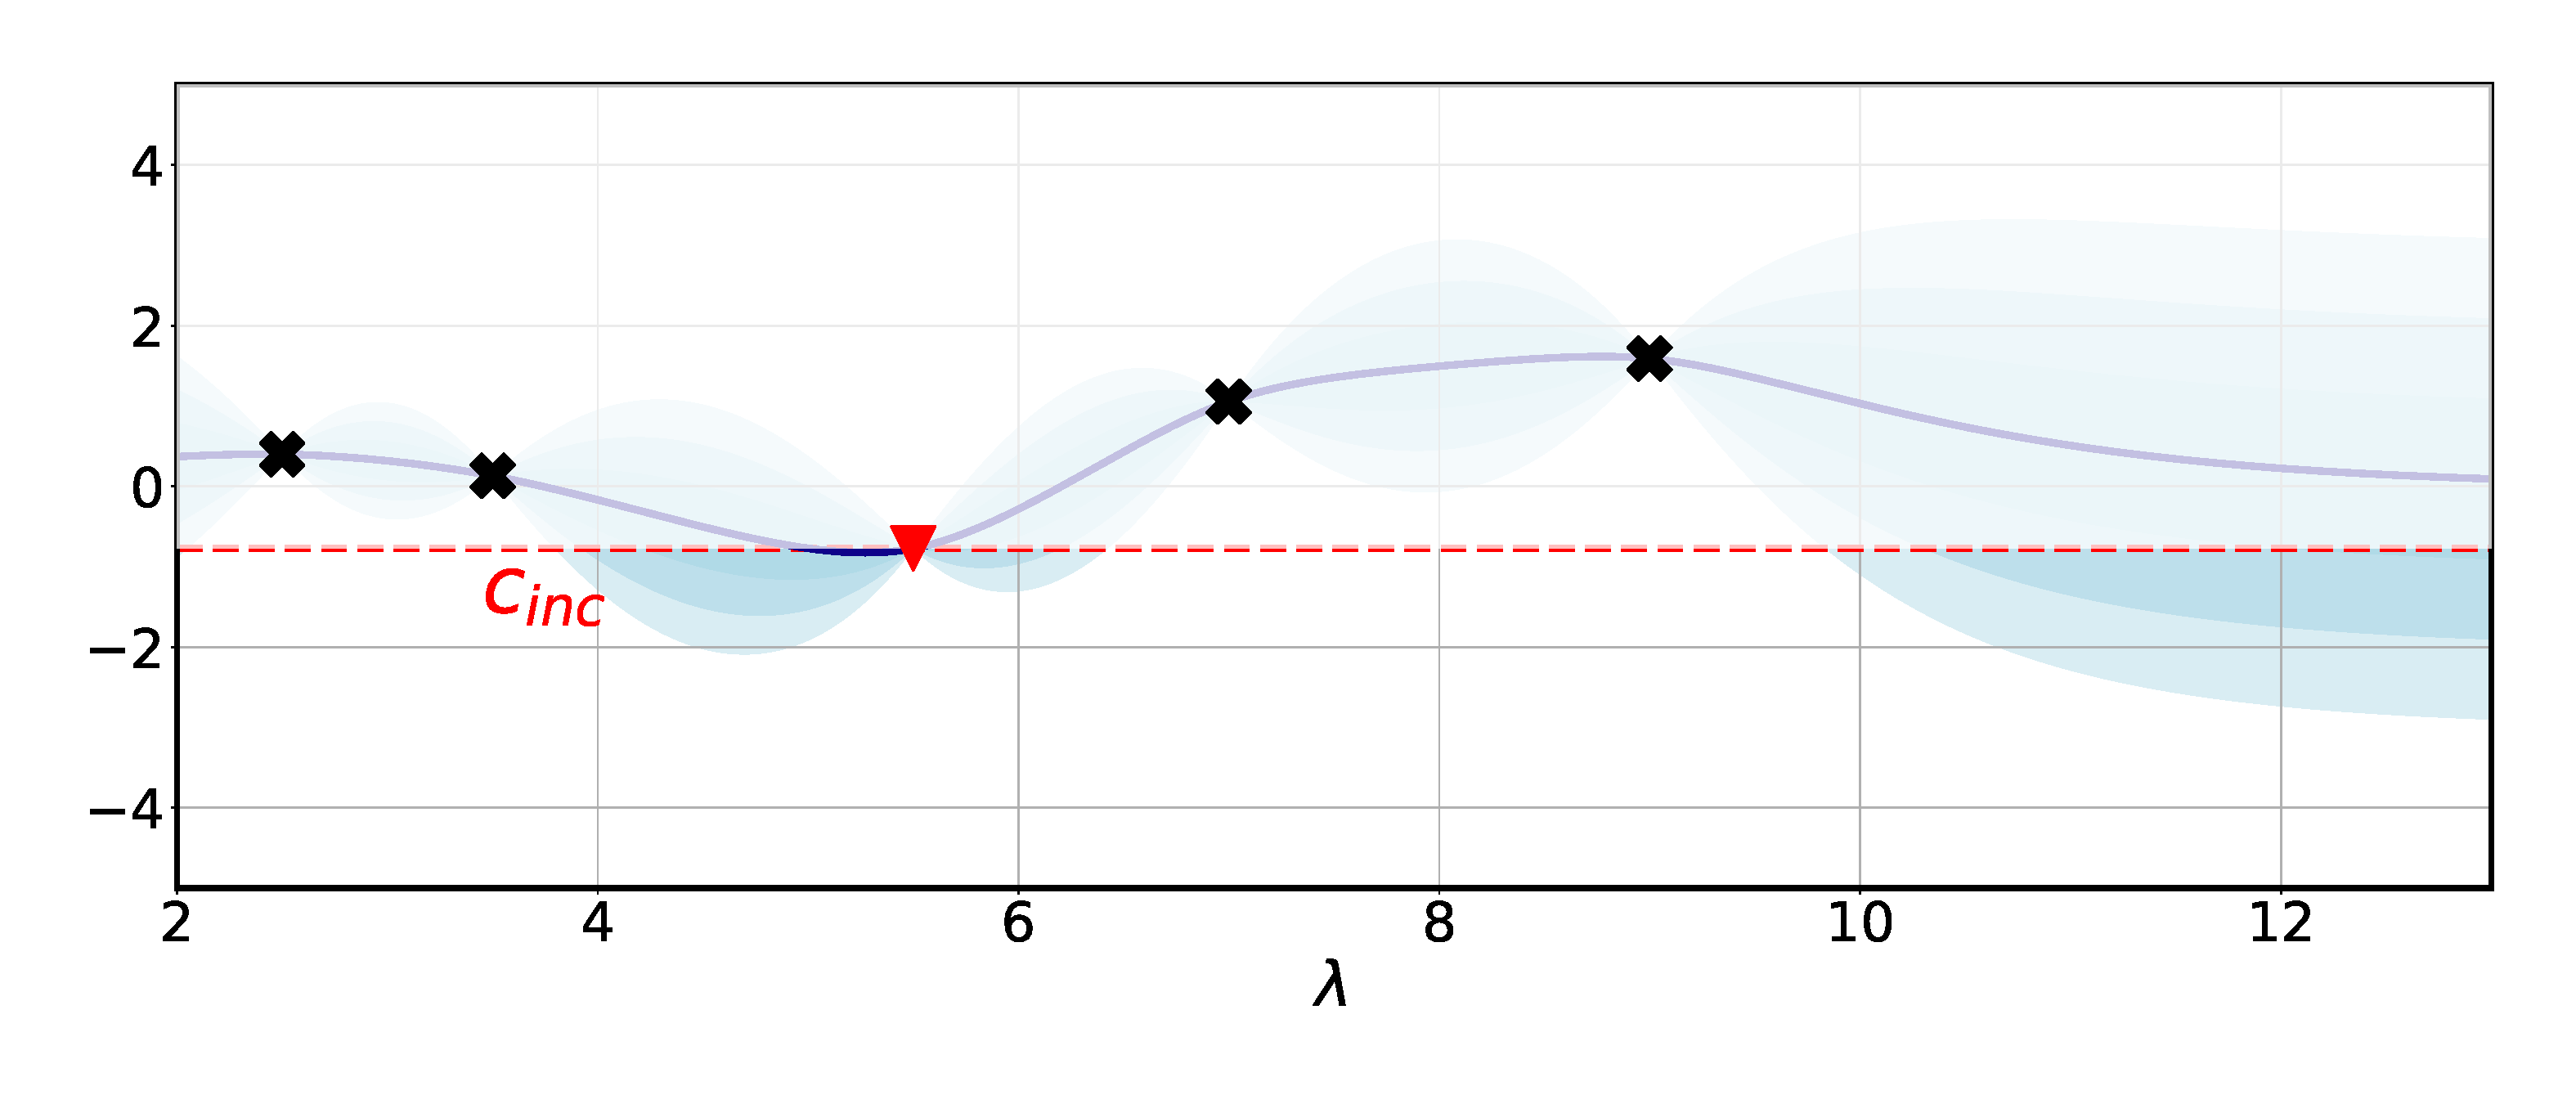
\includegraphics[width=\linewidth, height=0.7\textheight, keepaspectratio=true]{images/acq_func_images/pi/pi_4.pdf}};
        \node<.> [below=-1.0\belowcaptionskip of img4, align=center]{Intuitively, we care about the probability of improving over the current incumbent};
        \comment{We cannot be absolutely certain if there will be an improvement, but we are certain that if there is to be improvement, it is only possible in this zone.}
    
        \node<+> (img5) {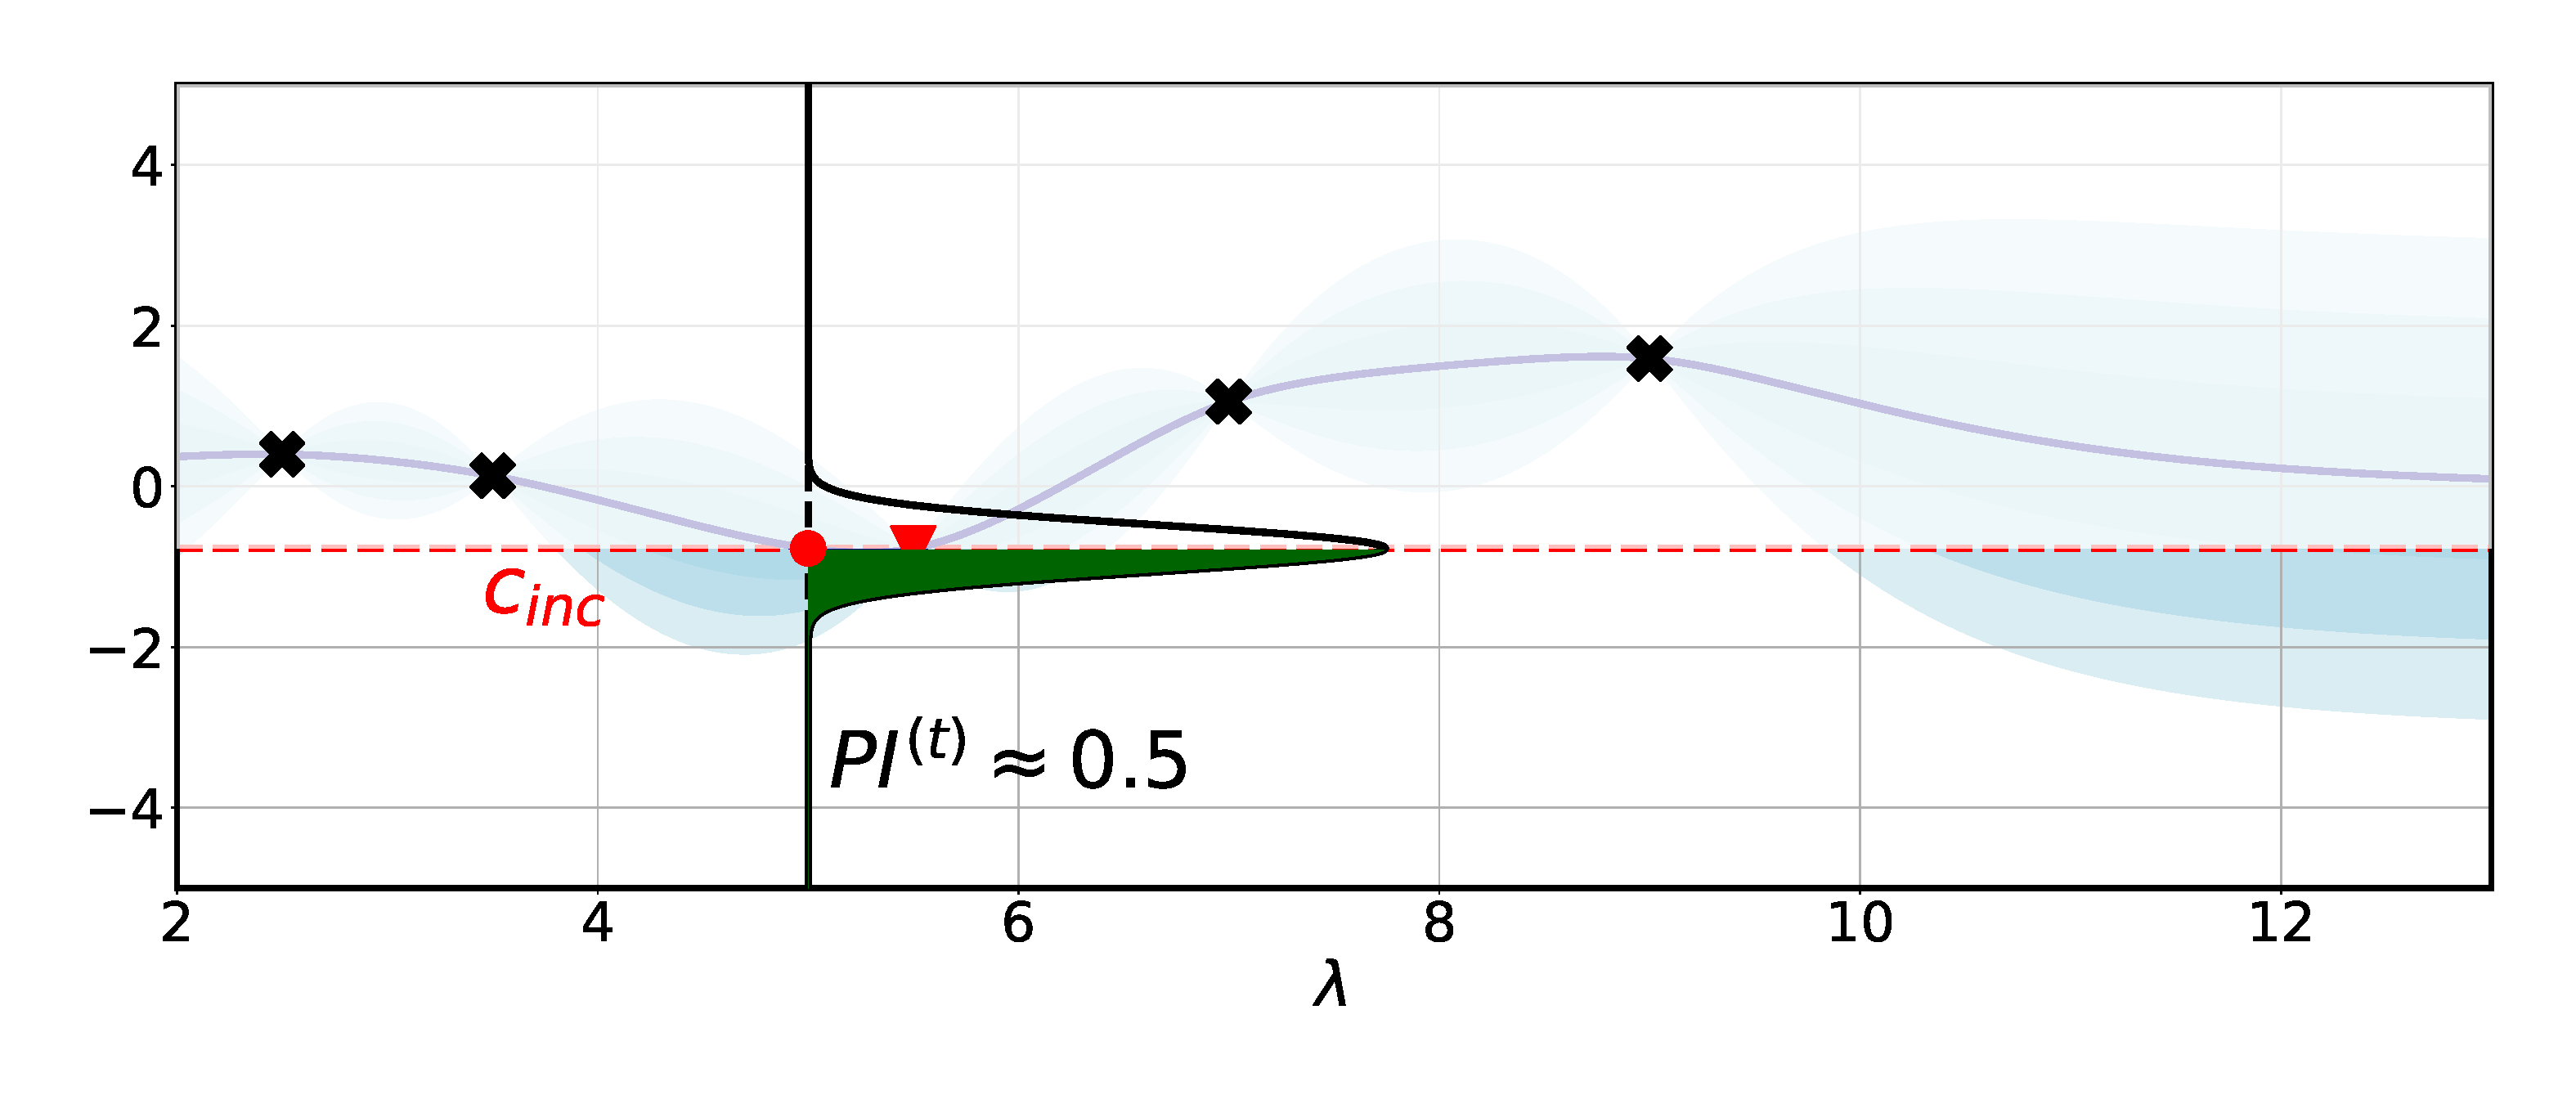
\includegraphics[width=\linewidth, height=0.7\textheight, keepaspectratio=true]{images/acq_func_images/pi/pi_5.pdf}};
        \node<.> [below=0.01\belowcaptionskip of img5, align=center]{PDF of a good candidate configuration. Only the green area is an improvement.};
    
        \node<+> (img6) {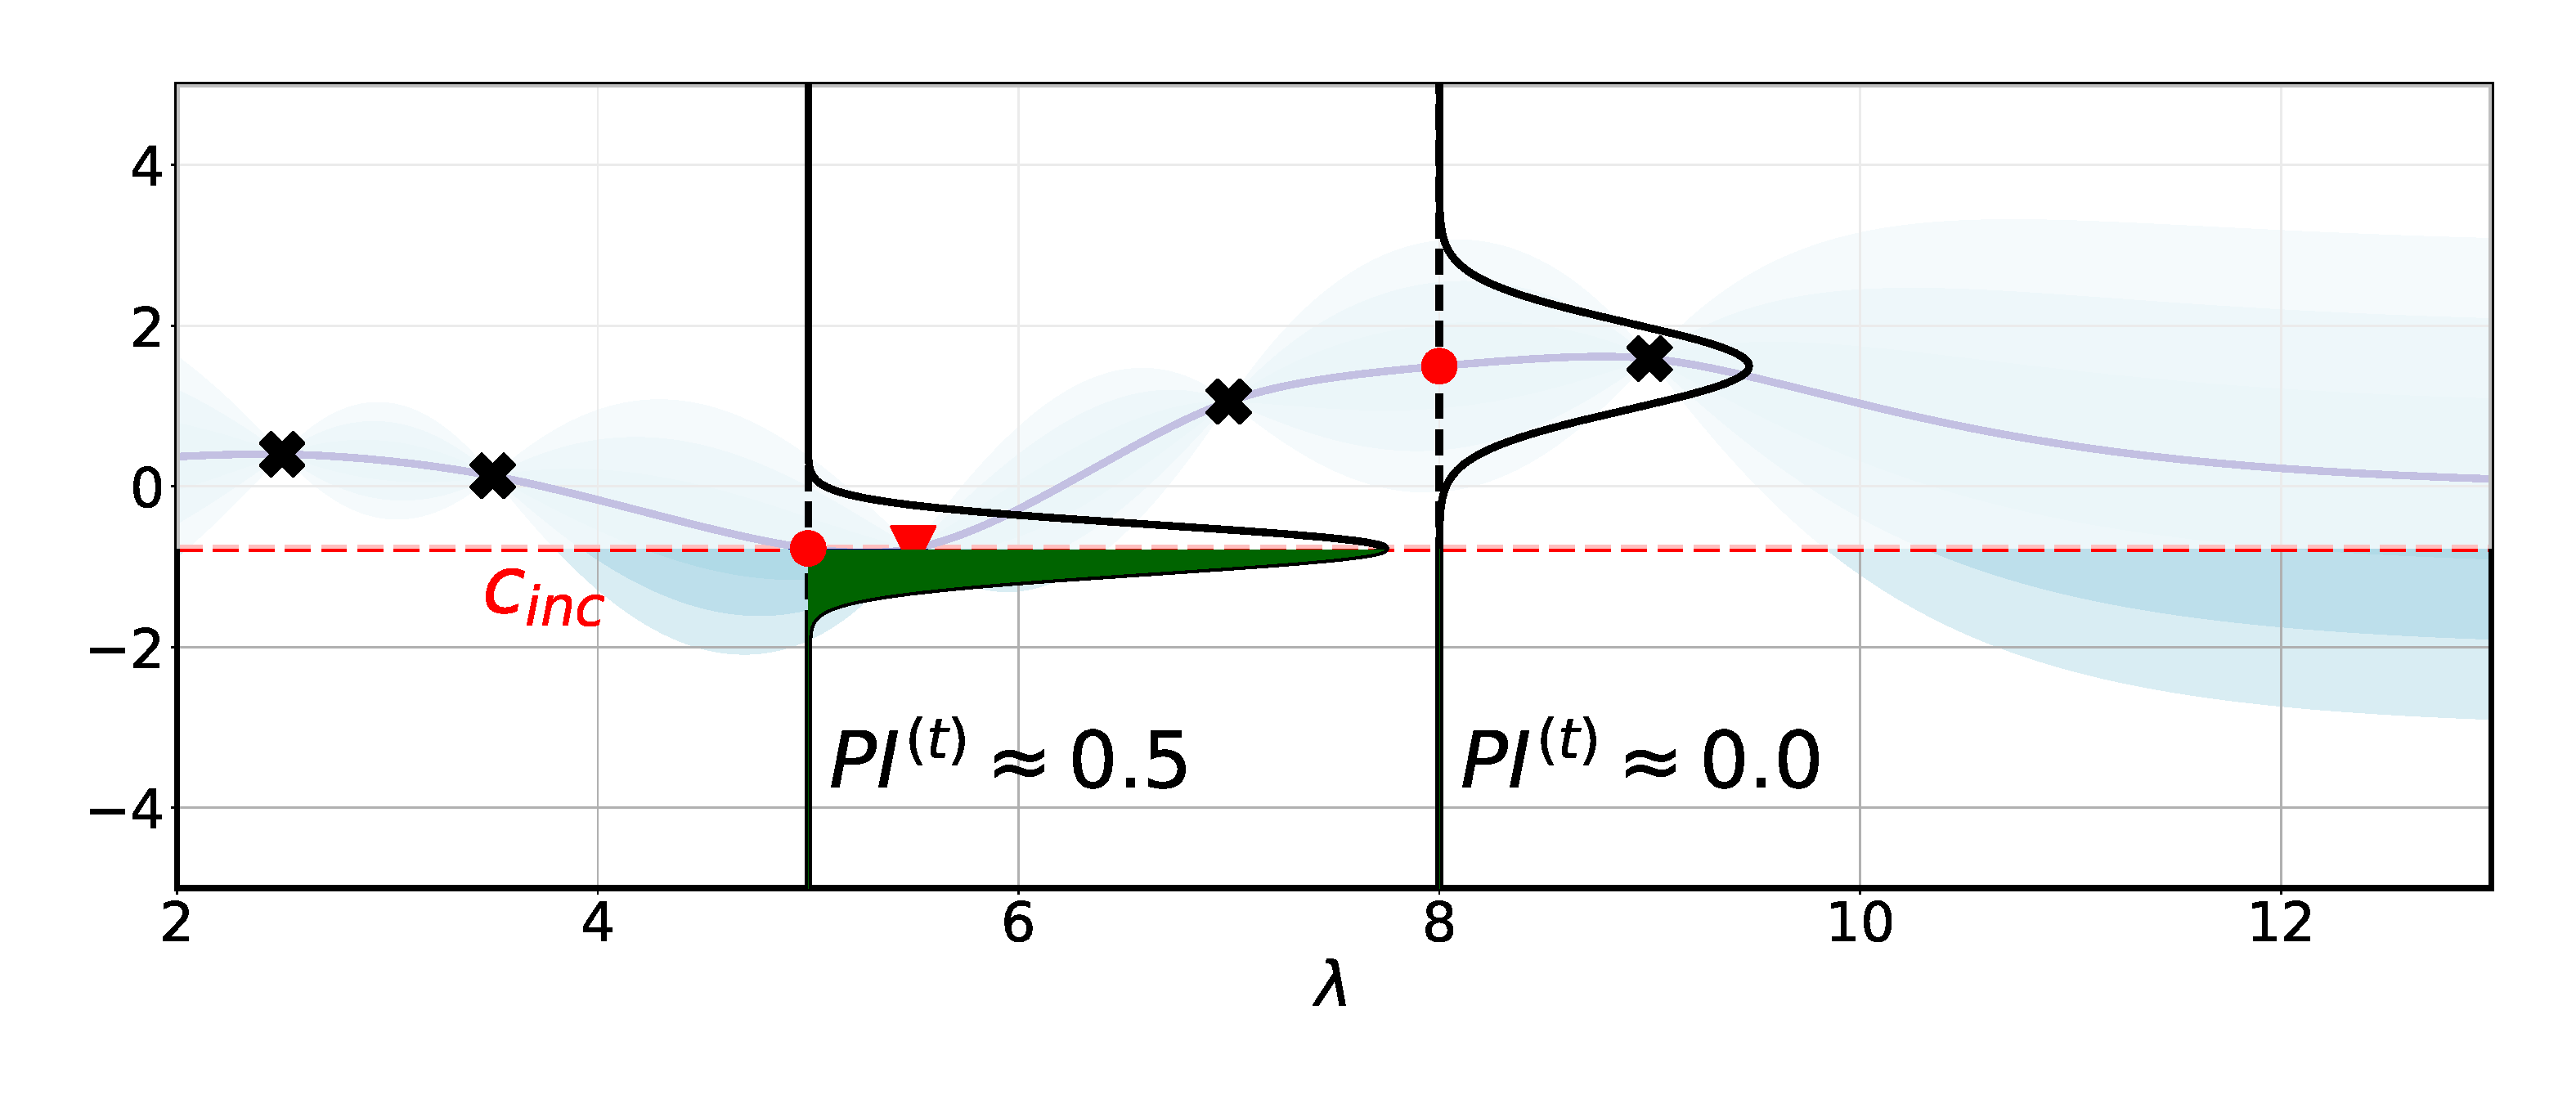
\includegraphics[width=\linewidth, height=0.7\textheight, keepaspectratio=true]{images/acq_func_images/pi/pi_6.pdf}};
        \node<.> [below=0.01\belowcaptionskip of img6, align=center]{PDF of a bad candidate configuration};
      \end{tikzpicture}
    % \end{figure}
}
% -----------------------------------------------------------------------
\begin{frame}[c]{Probability of Improvement (PI): Formal Definition}
%\framesubtitle{Probability of Improvement - Choosing a candidate}
%\comment{The definitions were adapted from the source to fit an acquisition function that is maximized and an objective function which is to be minimized.!}
\begin{itemize}
    \item We define the \alert{current incumbent at time step $t$} as: 
    $\incumbent[\bocount-1]\in\argmin_{\conf'\in\iter[\bocount-1]{\dataset}}\obs[\conf']$
    \item We write \alert{$\cost_{inc}$} shorthand for the \alert{cost of the current incumbent}: 
    $c_{inc} = \cost(\incumbent[\bocount-1])$
\smallskip
        \item The \alert{probability of improvement $\acq_{PI}(\conf)$} at a configuration $\conf$ is then defined as: 
        \alert{\[\iter{\acq}_{PI}(\conf) = P(\cost(\conf) \leq \cost_{inc}).\]}
    \vspace*{-0.5cm}
    \pause
    \item Since the predictive distribution for $\cost(\conf)$ is a Gaussian $\normaldist(\iter[\bocount-1]{\mean}(\conf), \iter[\bocount-1]{\variance}(\conf))$, this can be written as:
    \[
        \alert{\iter{\acq}_{PI}(\conf) = \cdf[Z]}, \quad \text{with } Z = \dfrac{\cost_{inc} - \iter[\bocount-1]{\mean}(\conf) - \xi}{\iter[\bocount-1]{\stddev}(\conf)}, 
    \]
    \newline
    where $\cdf(\cdot)$ is the CDF of the standard normal distribution and $\xi$ is an optional exploration parameter
    \pause
    \item[] \[\boxed{\text{Choose}\;\;\bonextsample \in \argmax_{\conf\in\pcs}(\iter{\acq}_{PI}(\conf))}\]
%    \comment{Source: Tutorial by Brochu et al.: https://arxiv.org/pdf/1012.2599.pdf }
\end{itemize}
\end{frame}
%-----------------------------------------------------------------------
\begin{frame}[t]{Expected Improvement (EI): Concept}
%\framesubtitle{Expected Improvement - Concept}

% \begin{figure}
  \centering
  \begin{tikzpicture}
    \node<+> (img1) {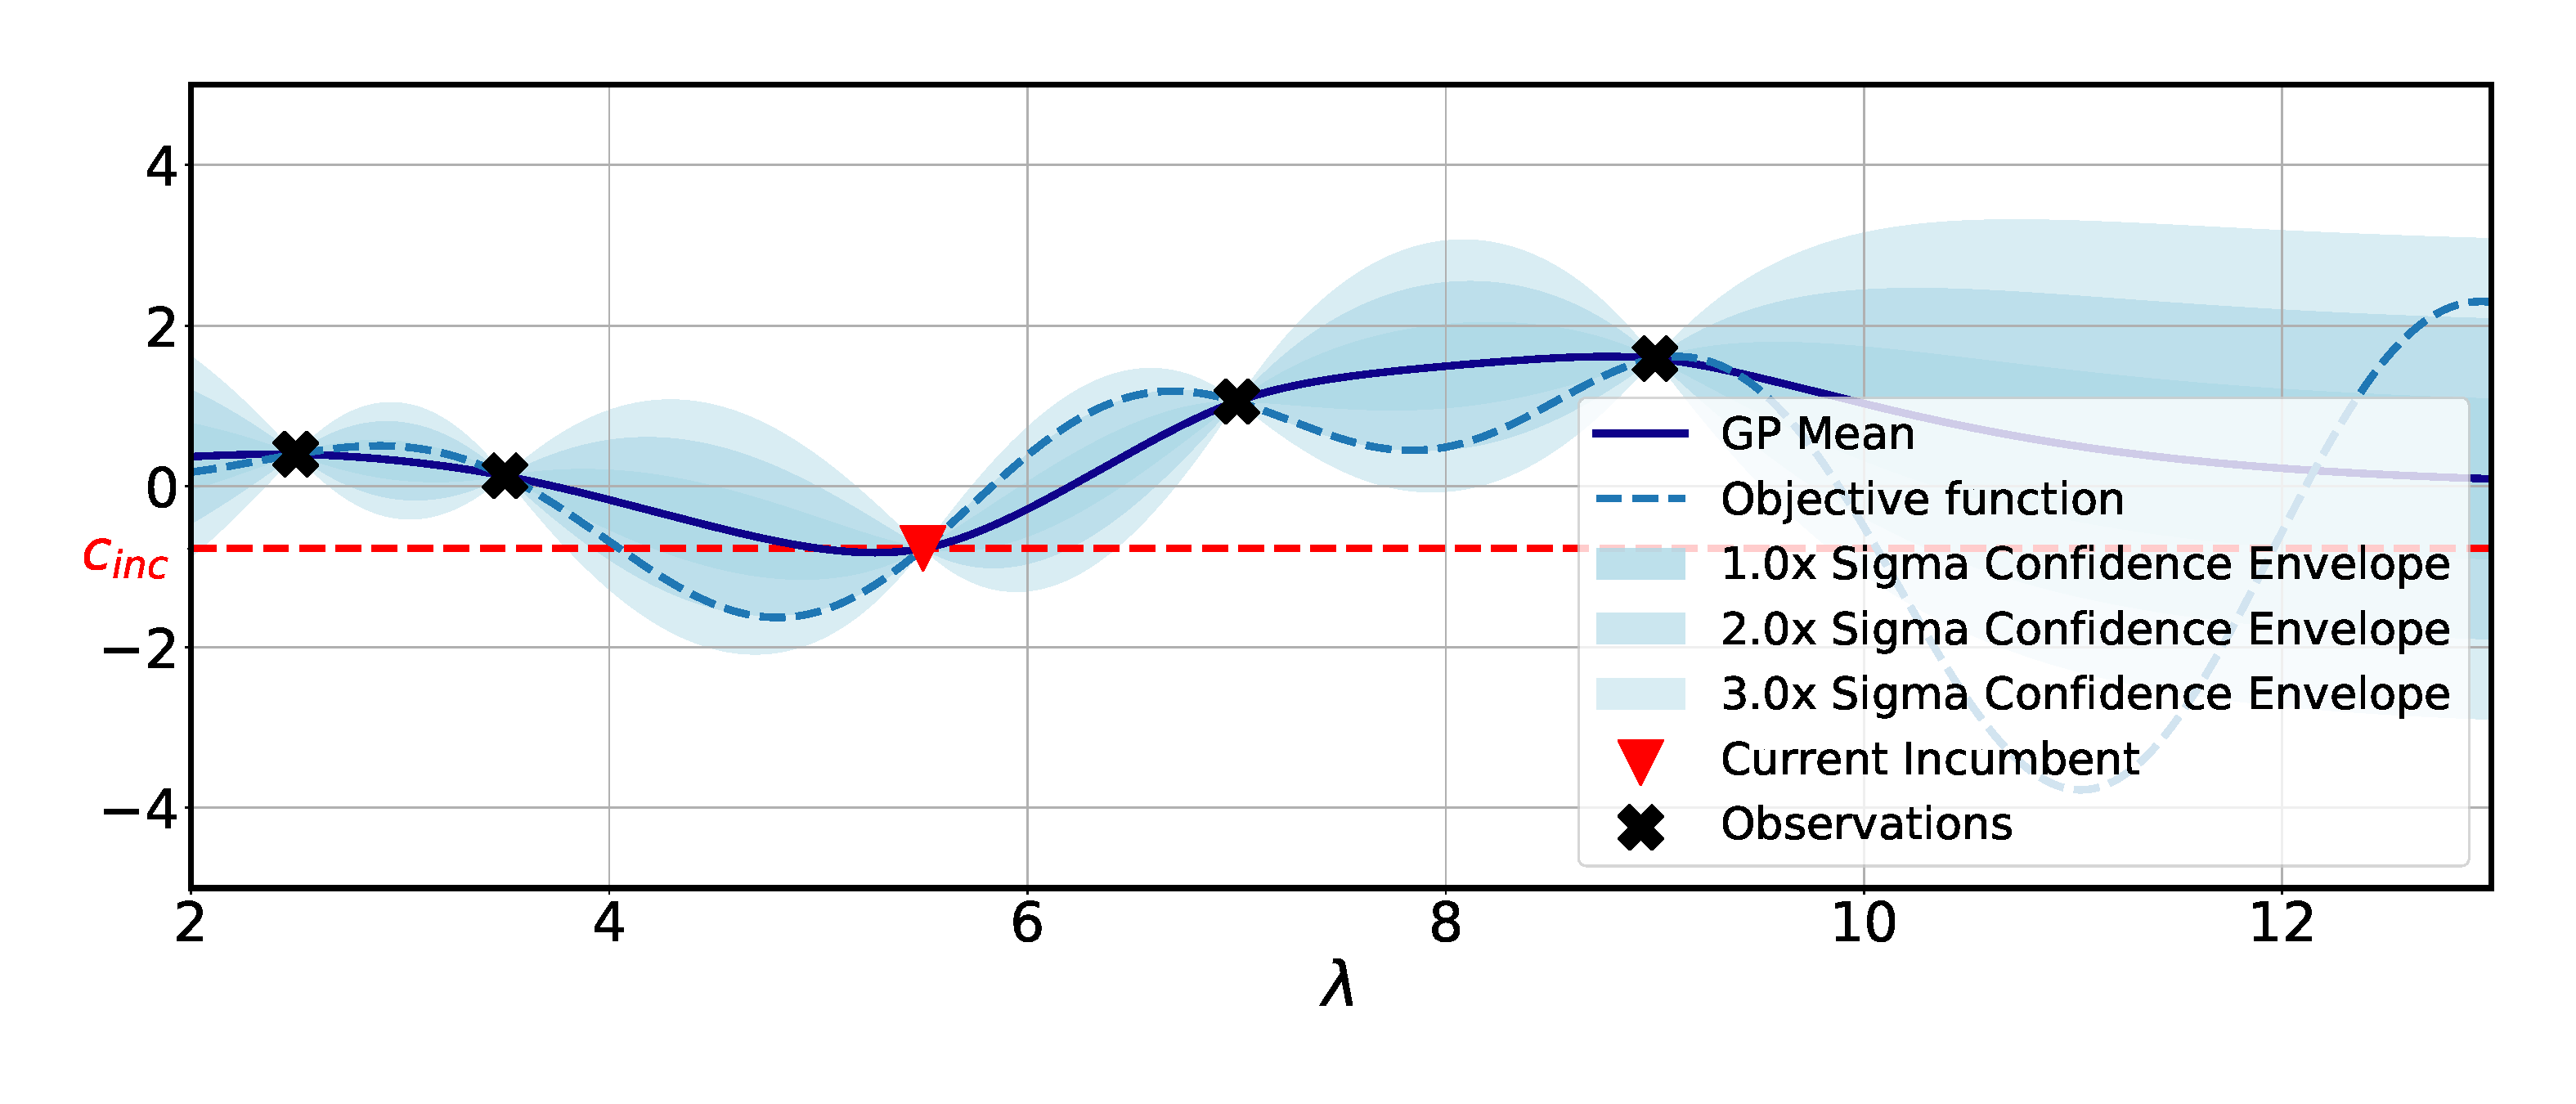
\includegraphics[width=\linewidth, height=0.7\textheight, keepaspectratio=true]{images/acq_func_images/ei/ei_1.pdf}};
    \node<.> [below=0.01\belowcaptionskip of img1, align=center]{Given the surrogate fit at iteration $\bocount$};

    \node<+> (img2a) {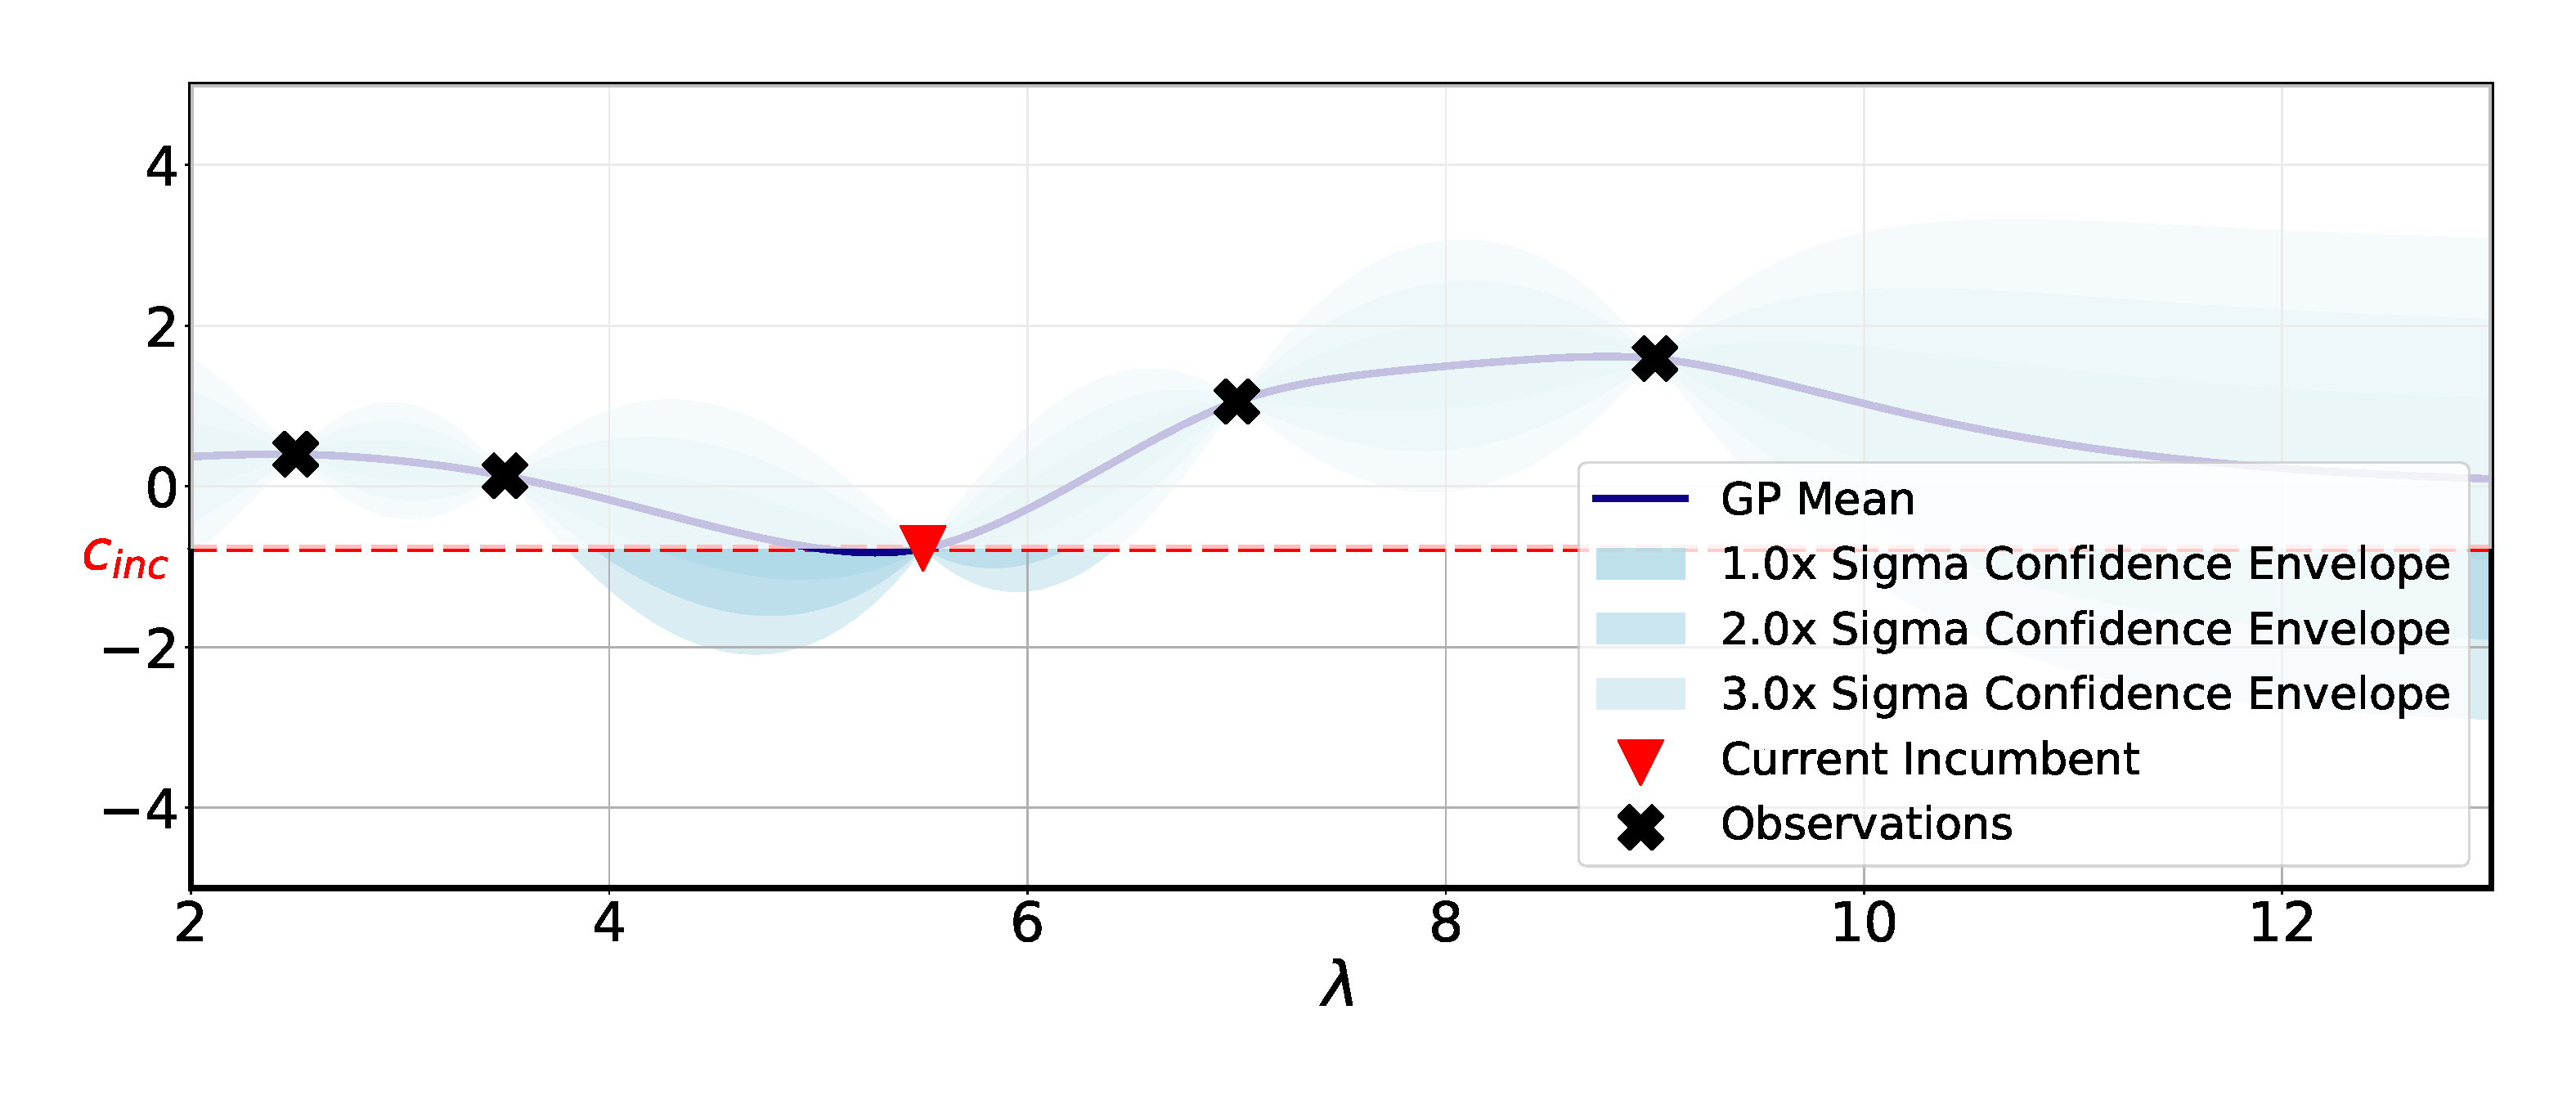
\includegraphics[width=\linewidth, height=0.7\textheight, keepaspectratio=true]{images/acq_func_images/ei/ei_2a.pdf}};
    \node<.> [below=0.01\belowcaptionskip of img2a, align=center]{Region of probable improvement -- but \alert{how large} is the improvement?};

    \node<+> (img2b) {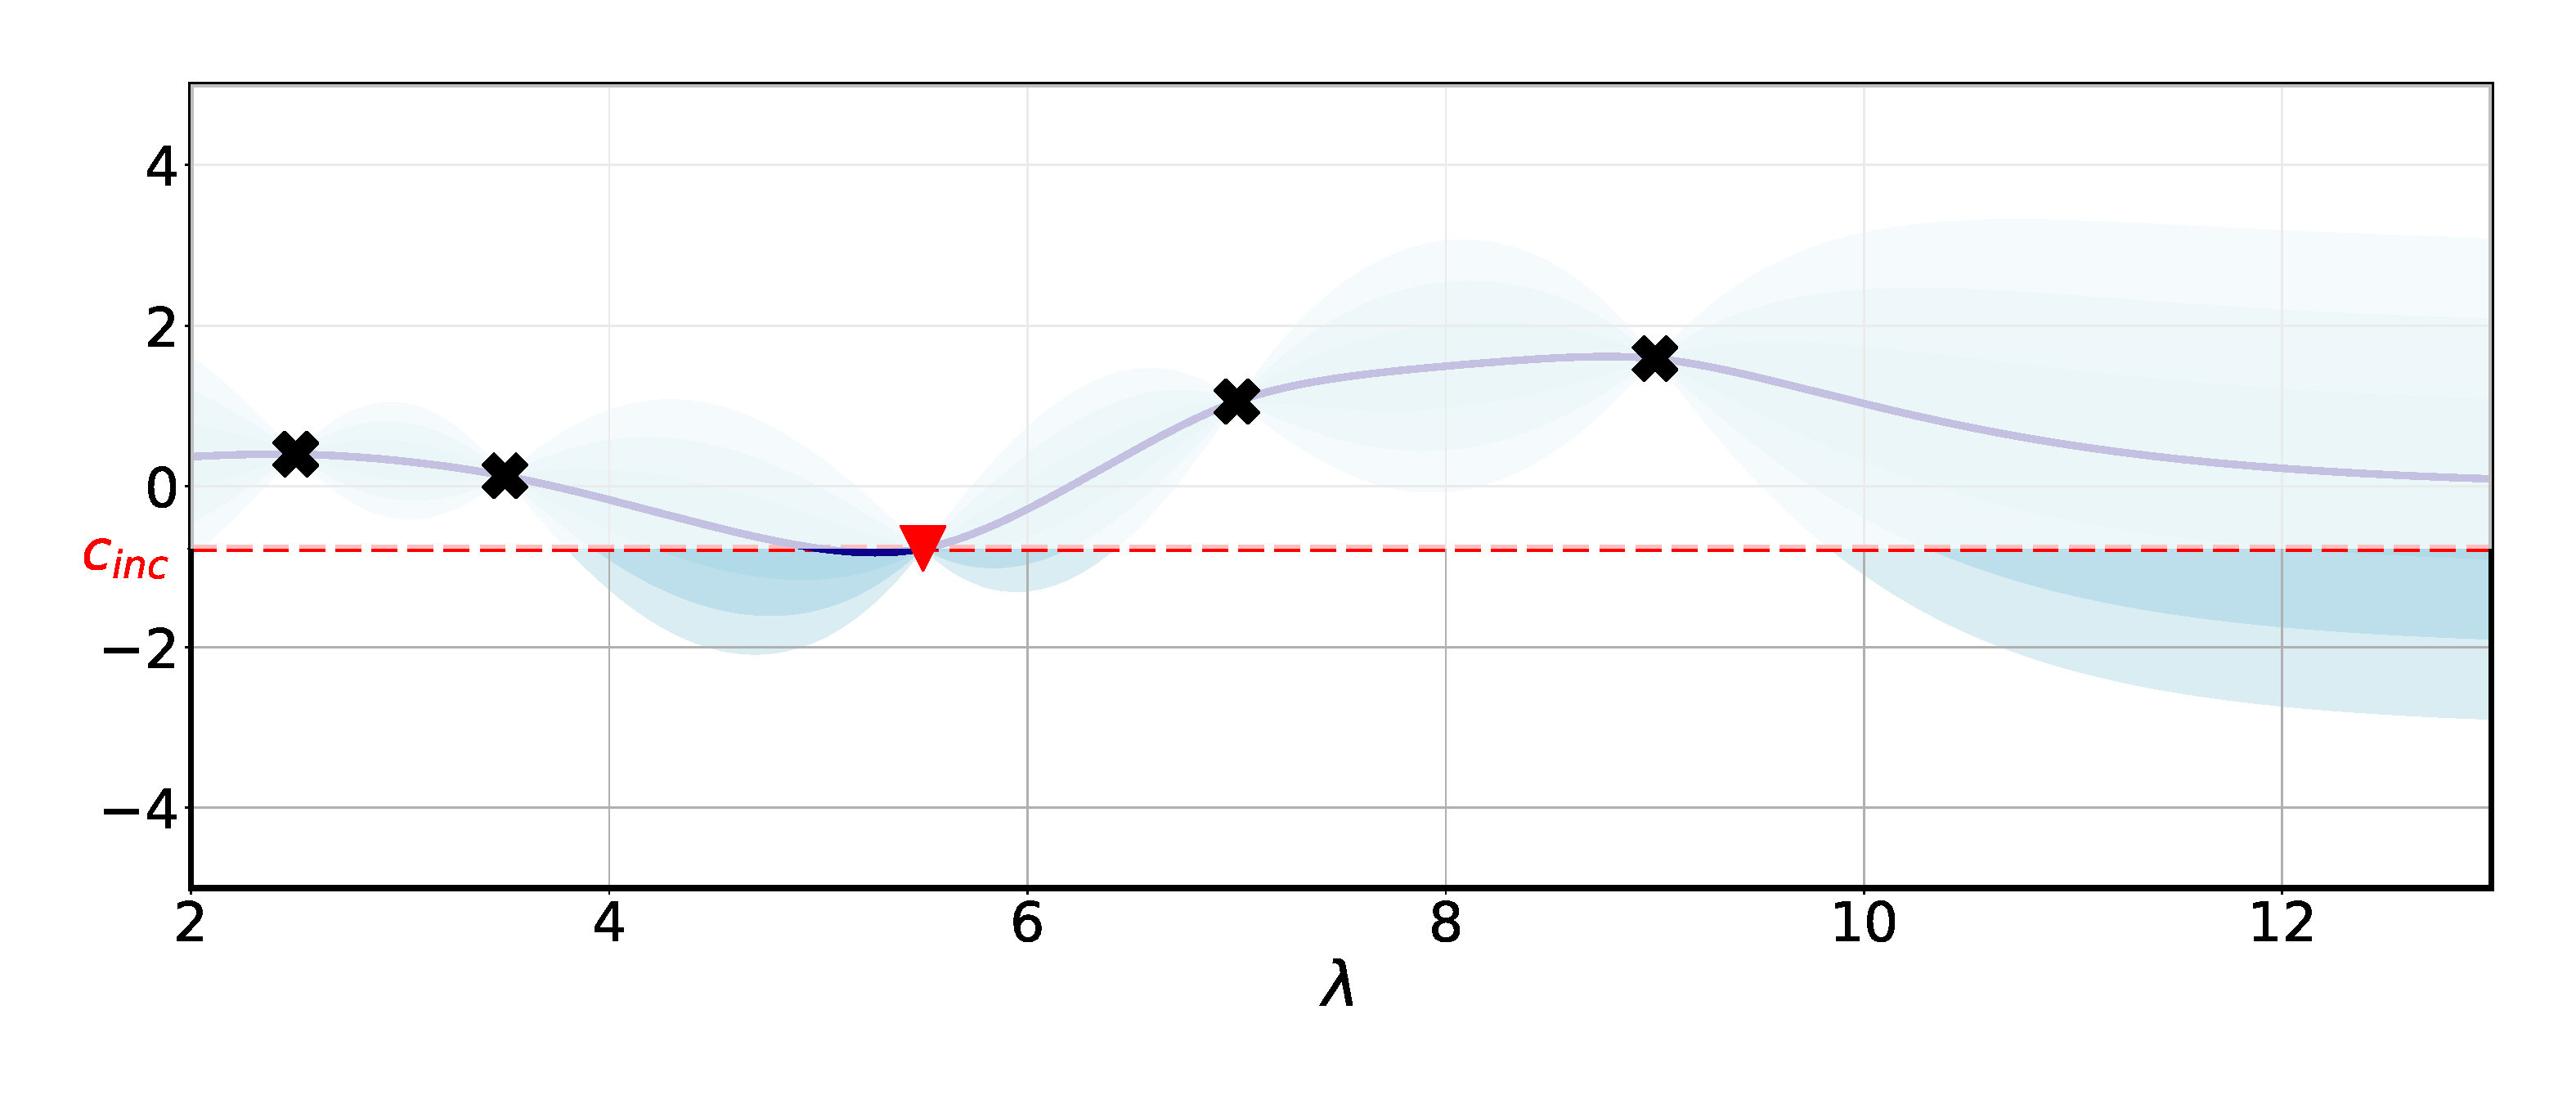
\includegraphics[width=\linewidth, height=0.7\textheight, keepaspectratio=true]{images/acq_func_images/ei/ei_2b.pdf}};
    \node<.> [below=0.01\belowcaptionskip of img2b, align=center]{Region of probable improvement -- but \alert{how large} is the improvement?};

    \node<+> (img3) {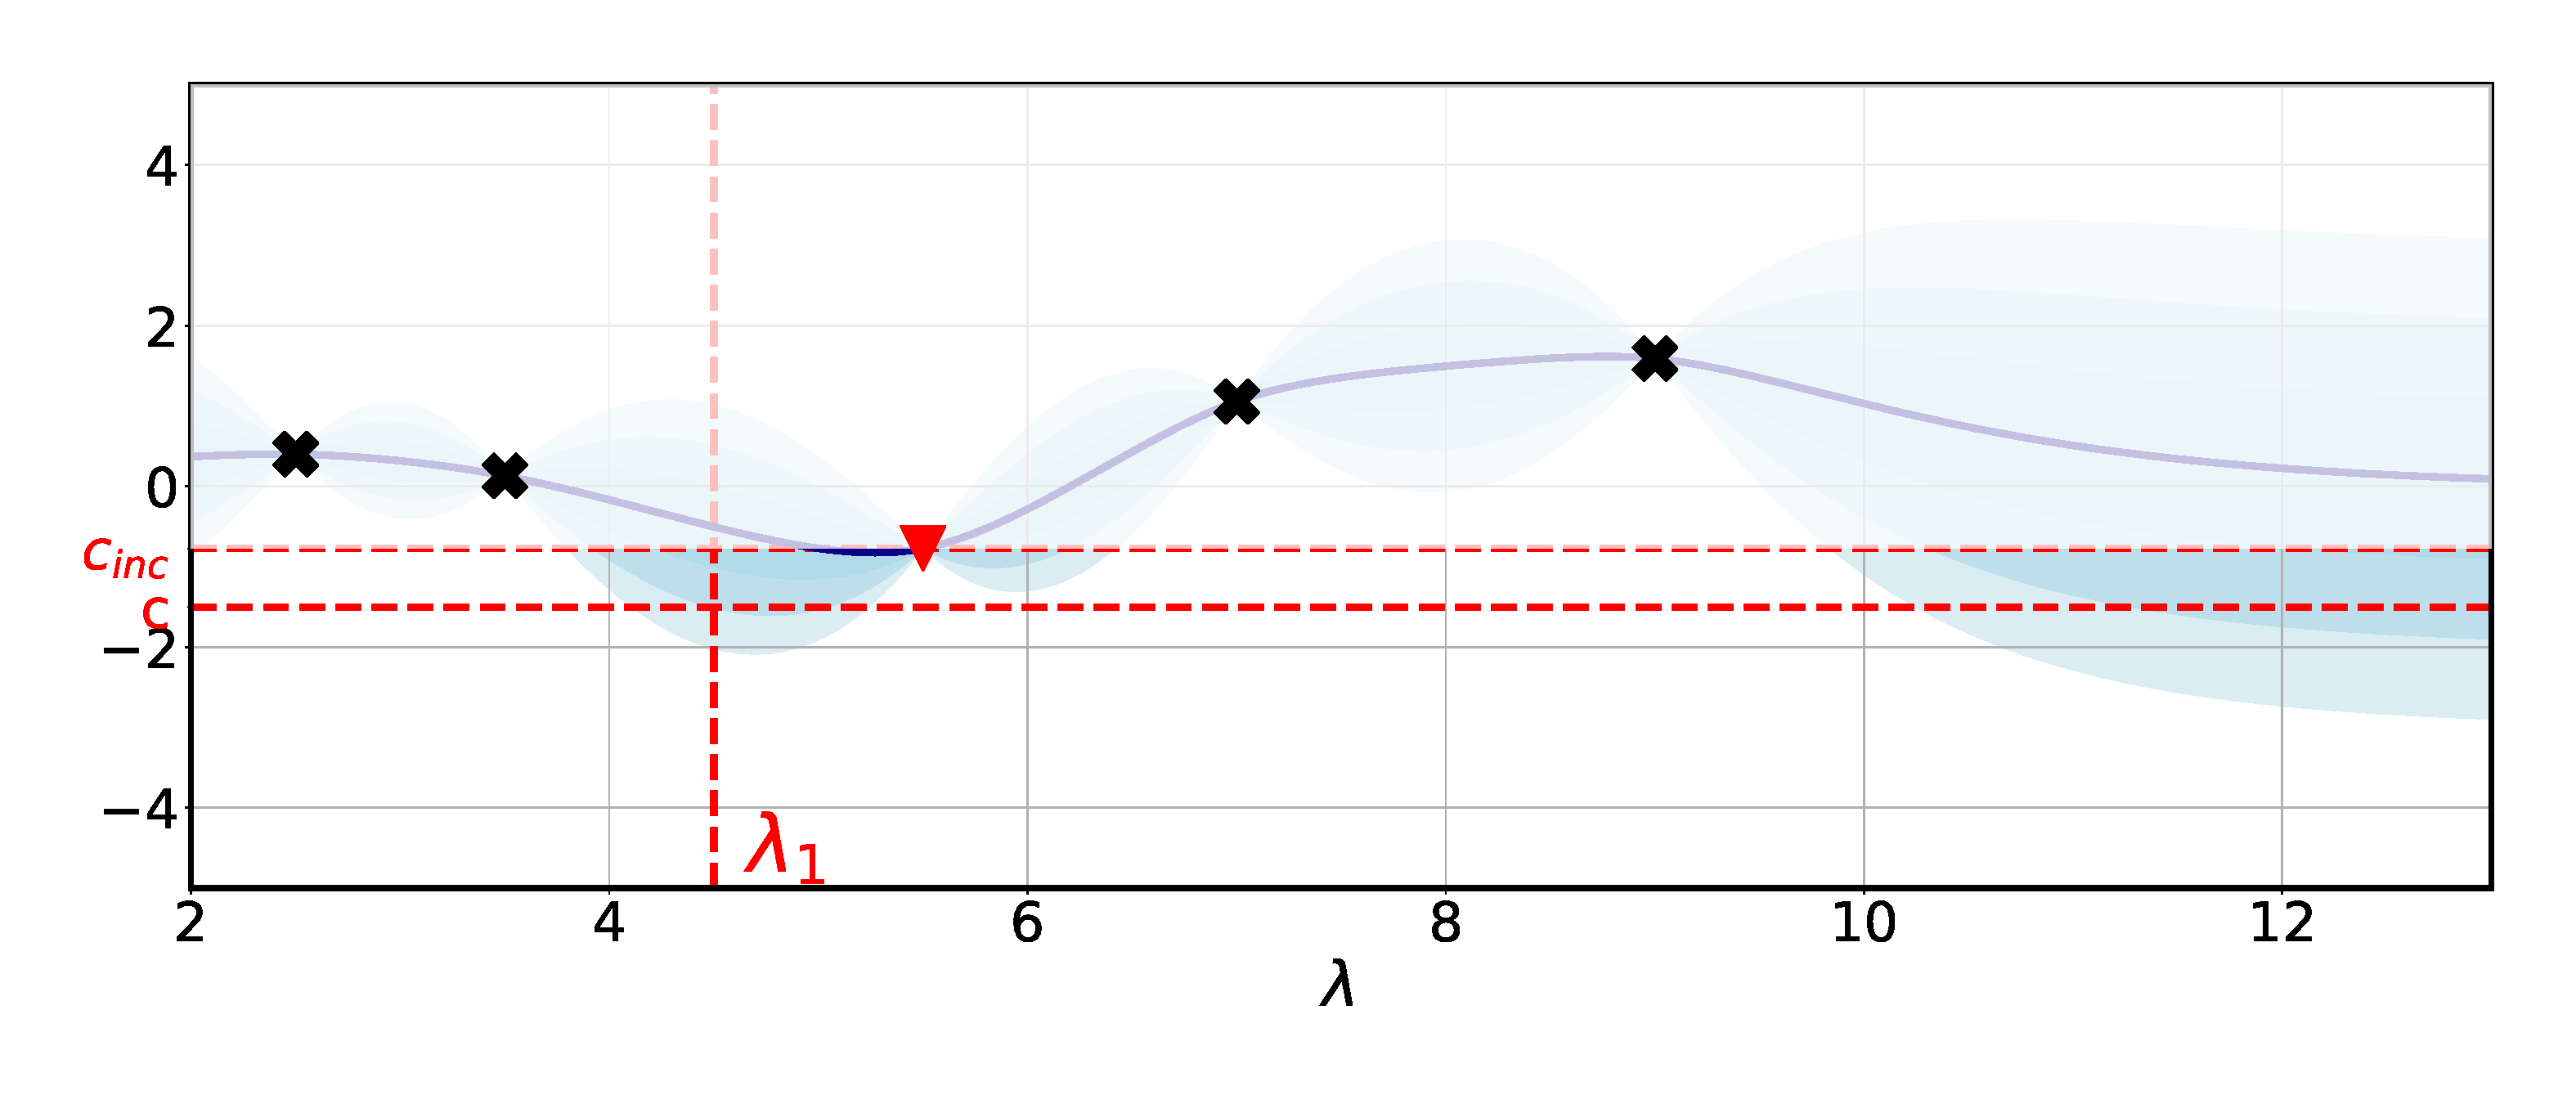
\includegraphics[width=\linewidth, height=0.7\textheight, keepaspectratio=true]{images/acq_func_images/ei/ei_3.pdf}};
    \node<.> [below=0.01\belowcaptionskip of img3, align=center]{Hypothetical \emph{real} cost $c$ at a given $\conf$ - unknown in practice without evaluating};

    \node<+> (img4) {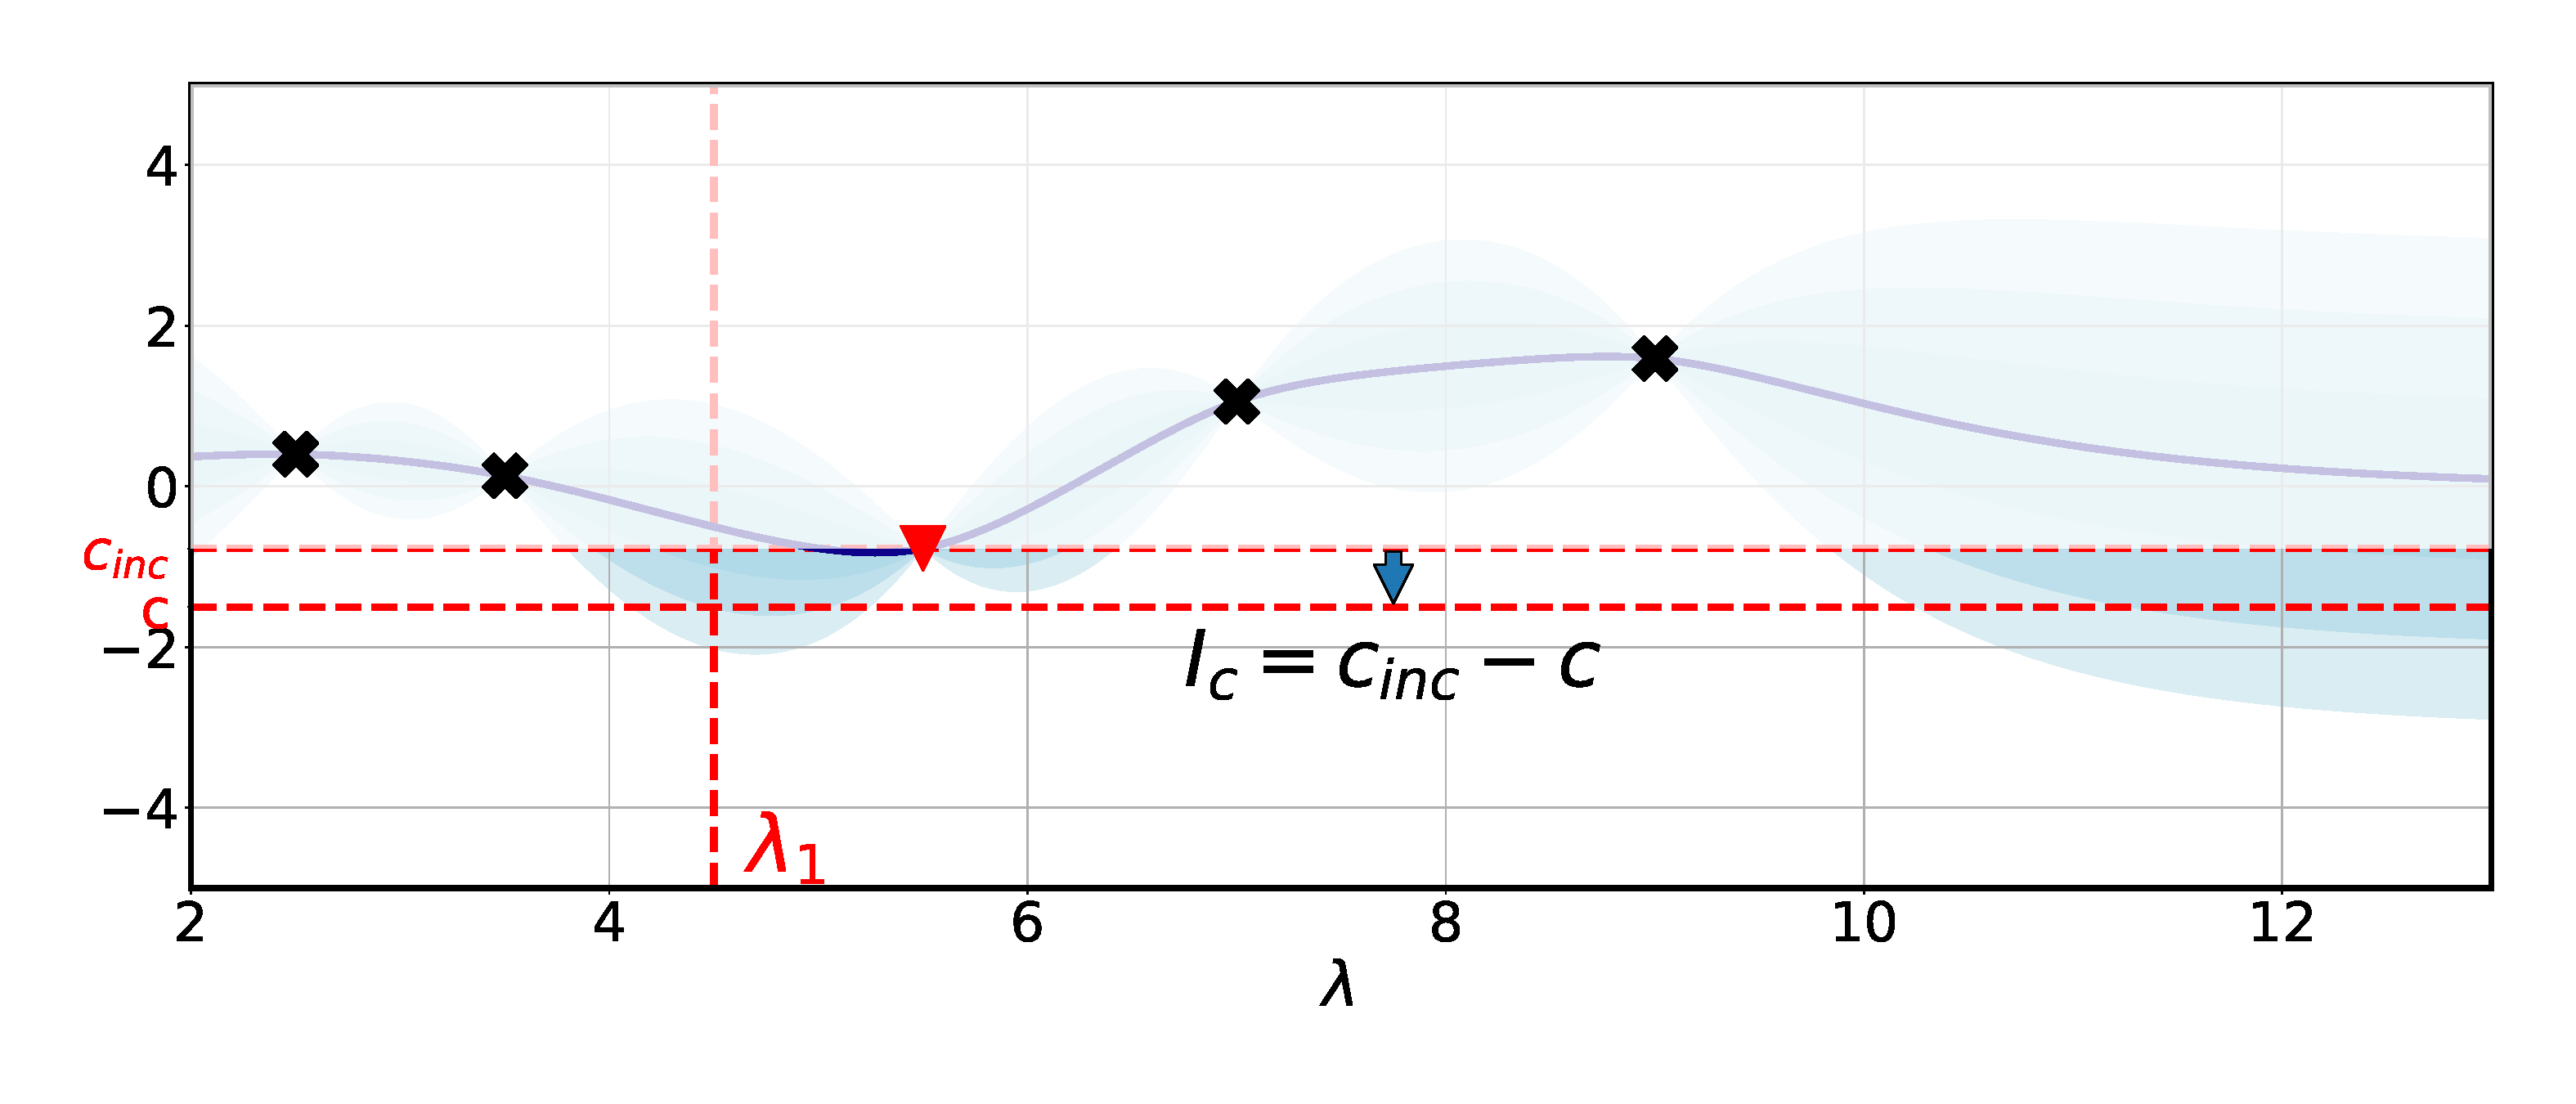
\includegraphics[width=\linewidth, height=0.7\textheight, keepaspectratio=true]{images/acq_func_images/ei/ei_4.pdf}};
    \node<.> [below=-0.01\belowcaptionskip of img4, align=center]{Given a hypothetical $c$, we can improve the improvement $I_c(\conf)$};
%    Without performing an actual evaluation, we cannot calculate $\iter{I}(\conf)$};

    \node<+> (img5) {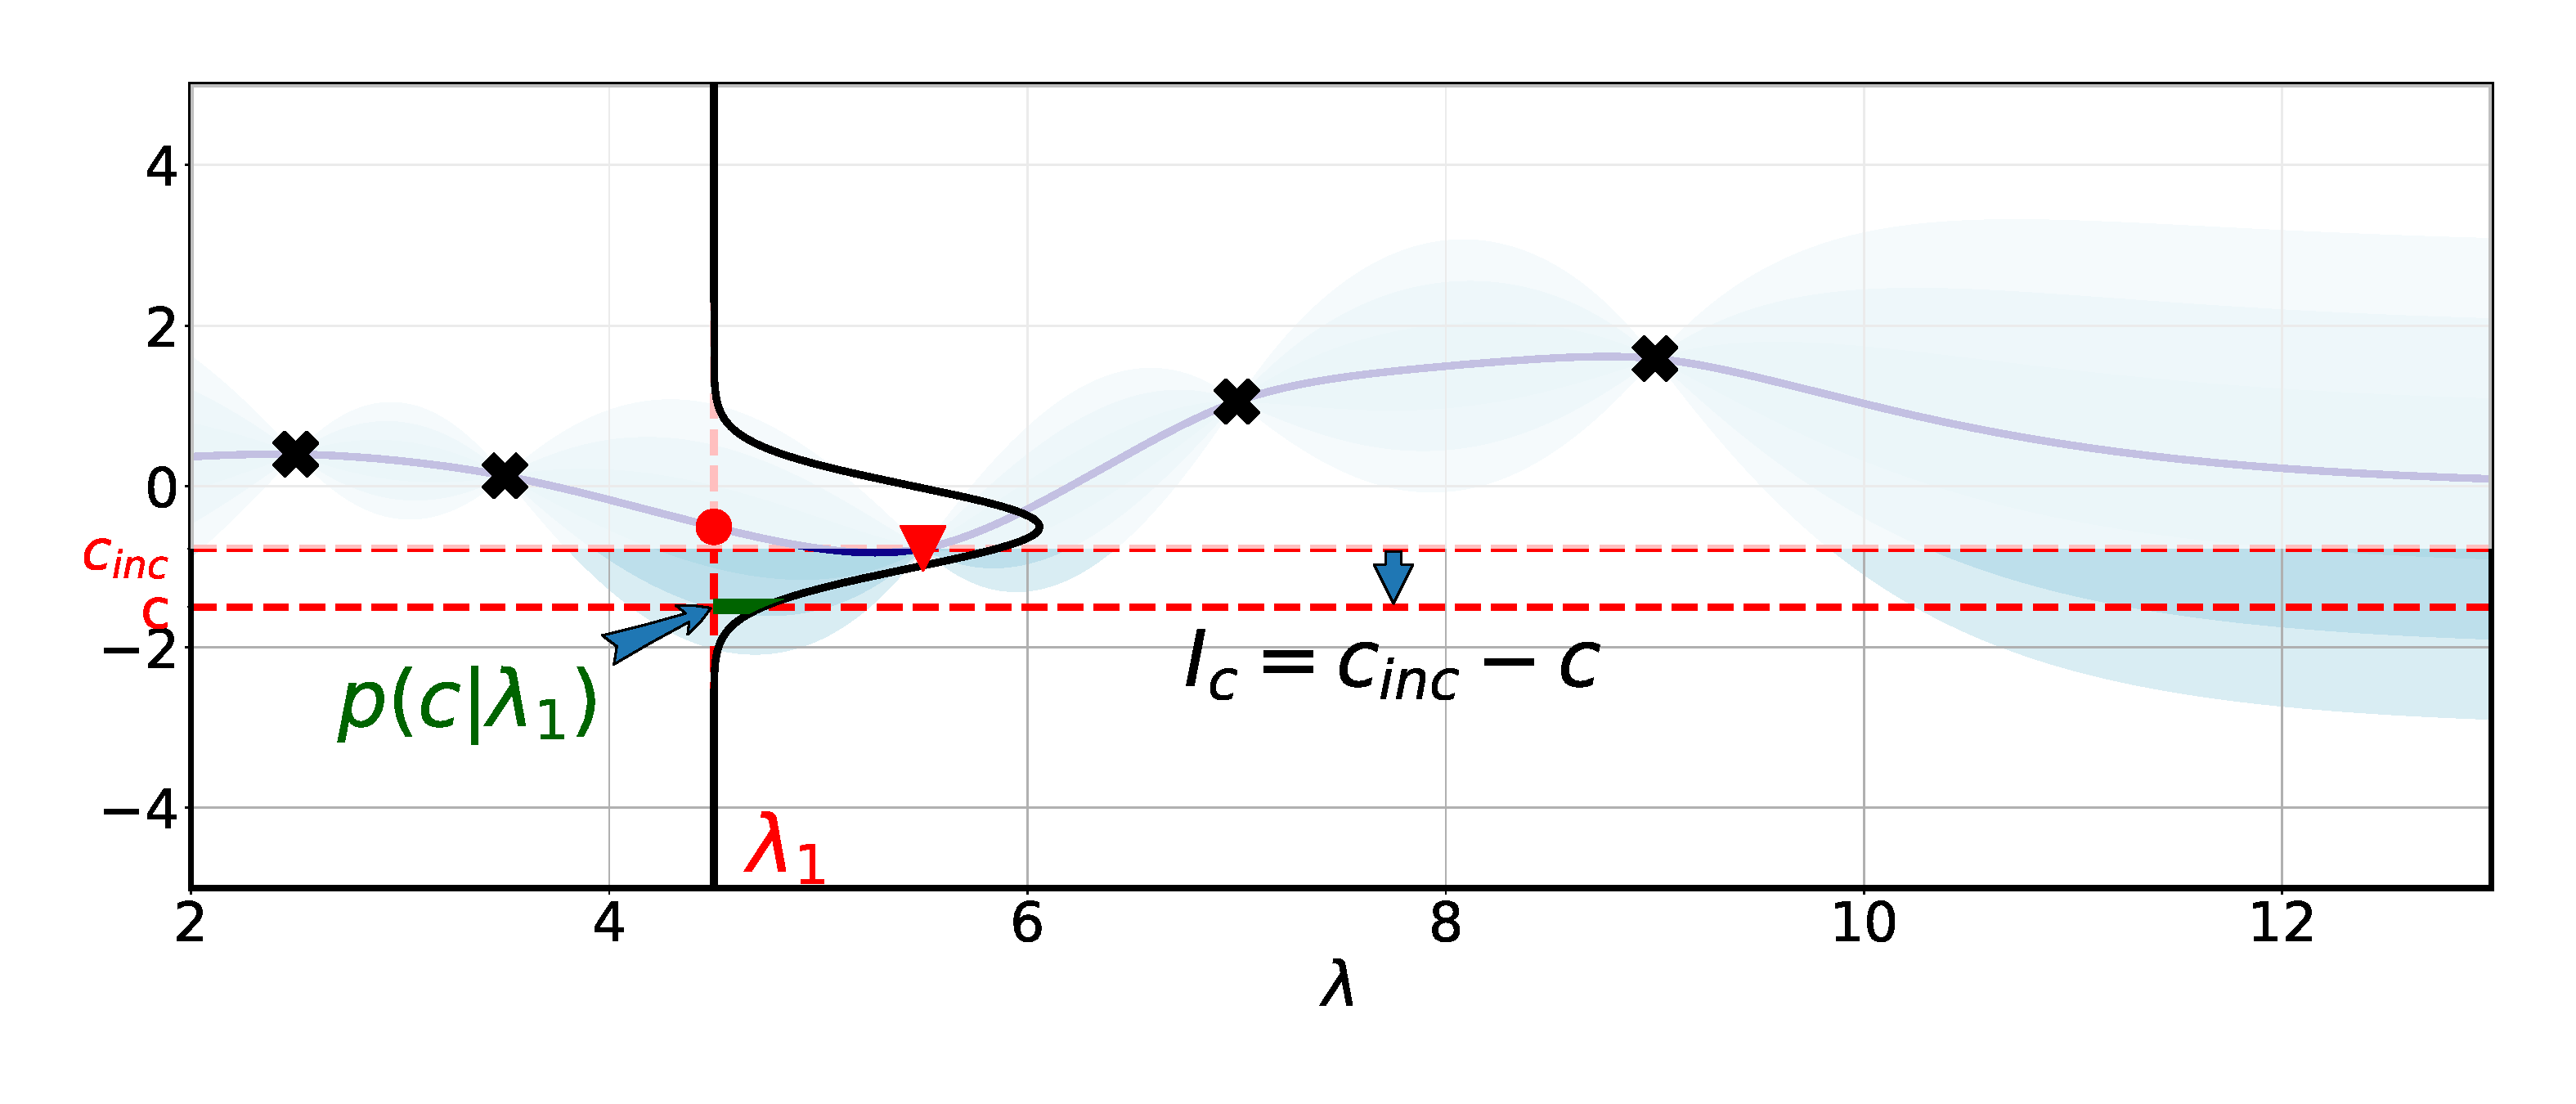
\includegraphics[width=\linewidth, height=0.7\textheight, keepaspectratio=true]{images/acq_func_images/ei/ei_5.pdf}};
    \node<.> [below=0.01\belowcaptionskip of img5, align=center]{Given $\surro(\conf) = \normaldist( \mean(\conf), \variance(\conf))$, we can also compute $p(\cost|\conf)$.};

    \node<+> (img6) {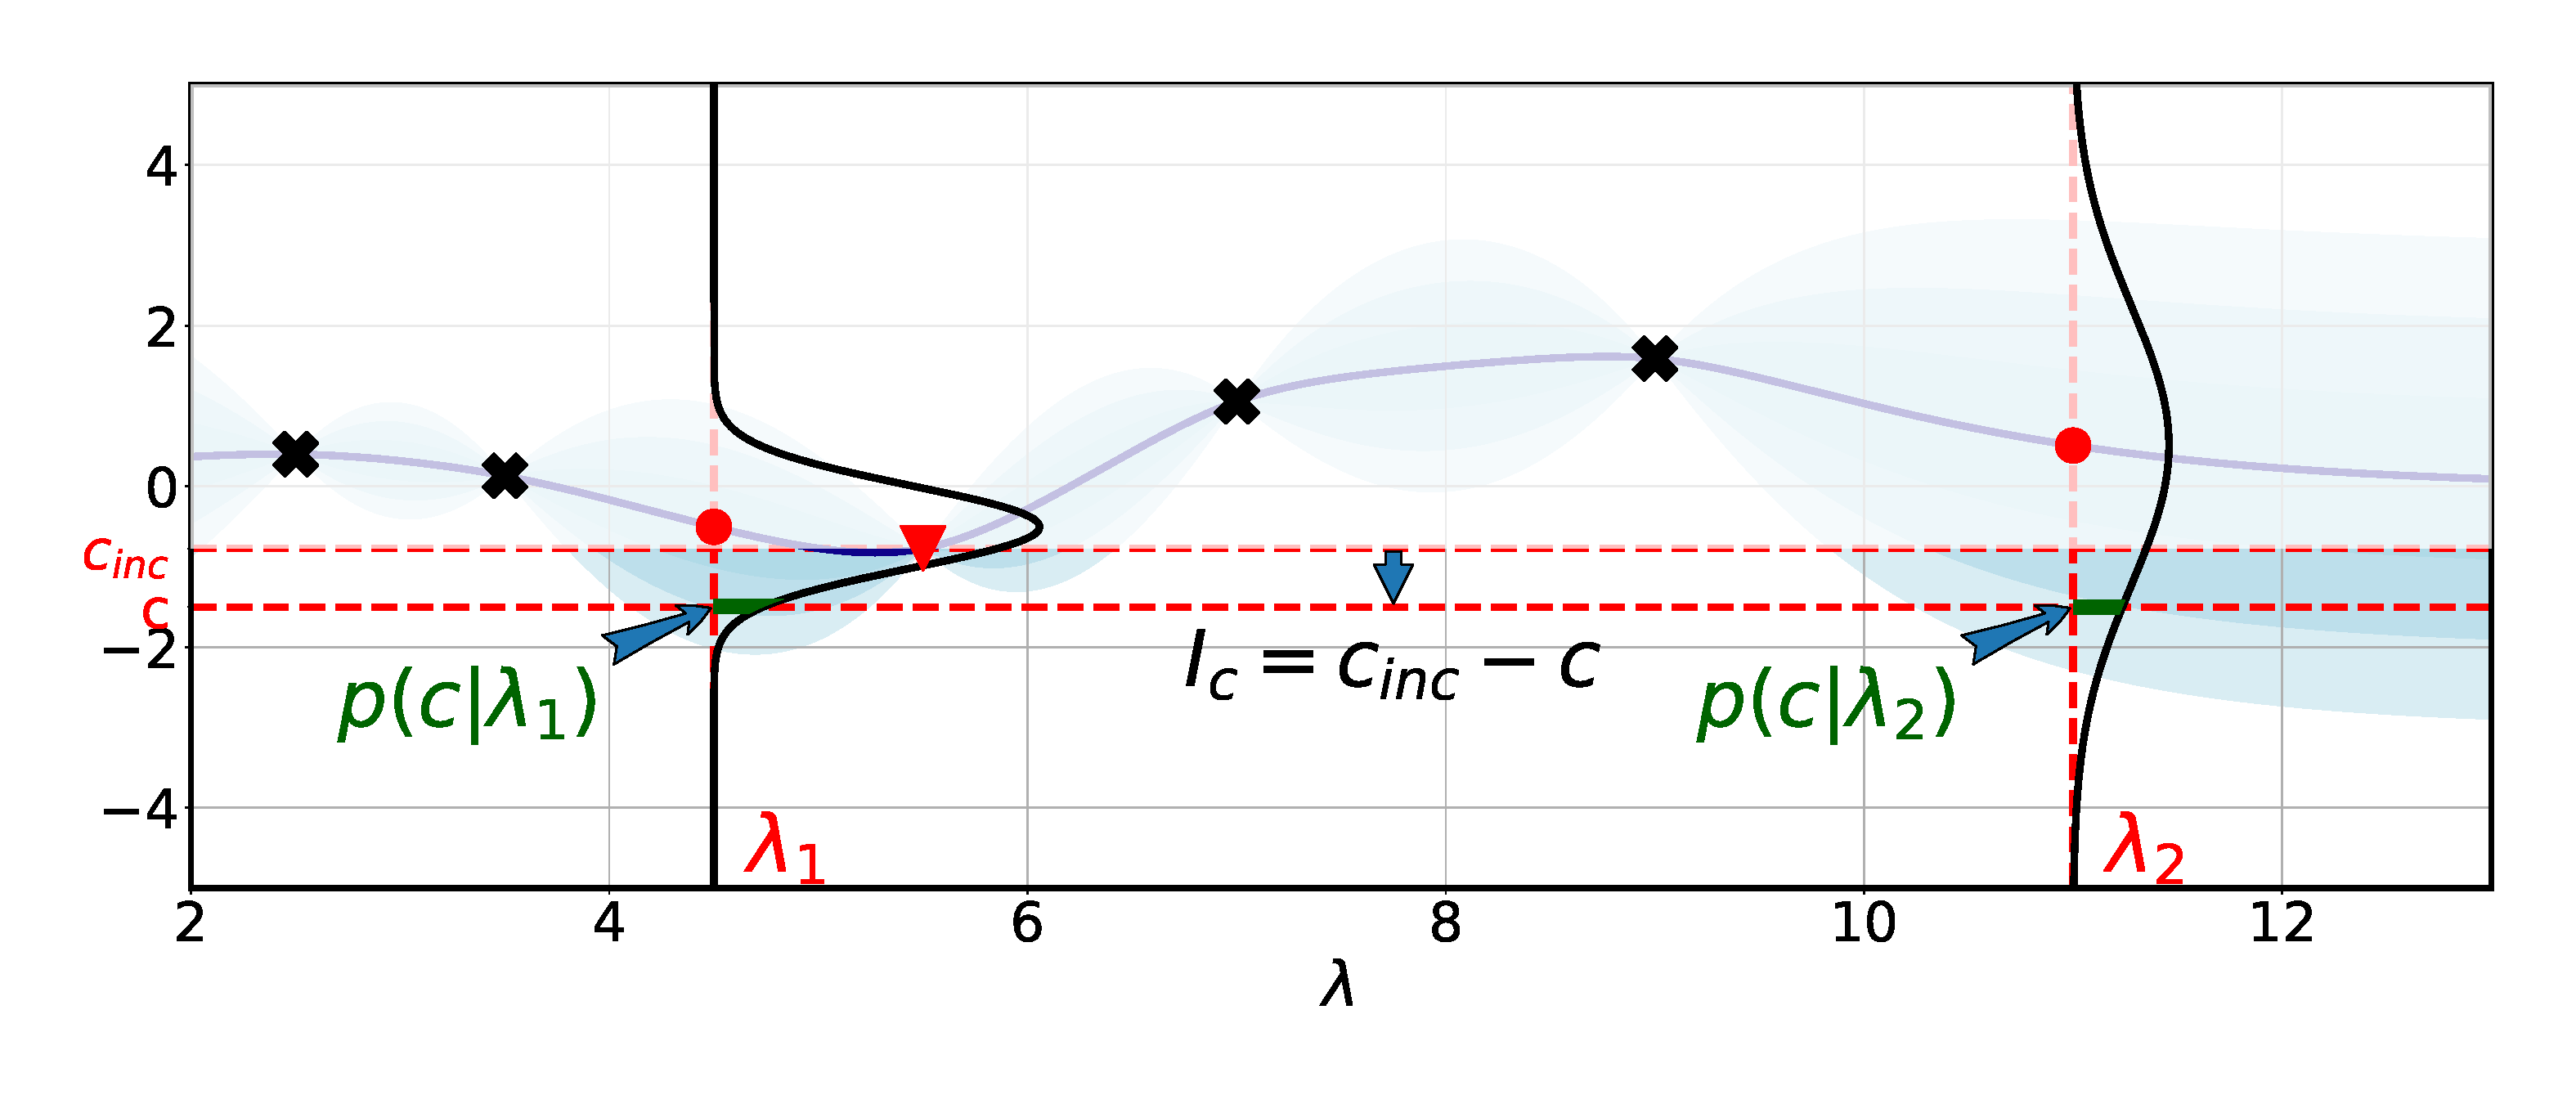
\includegraphics[width=\linewidth, height=0.7\textheight, keepaspectratio=true]{images/acq_func_images/ei/ei_6.pdf}};
    \node<.> [below=-0.01\belowcaptionskip of img6, align=center]{Compare the likelihood of a given improvement for two different configurations $\conf_1$ and $\conf_2$};

    \node<+> (img7) {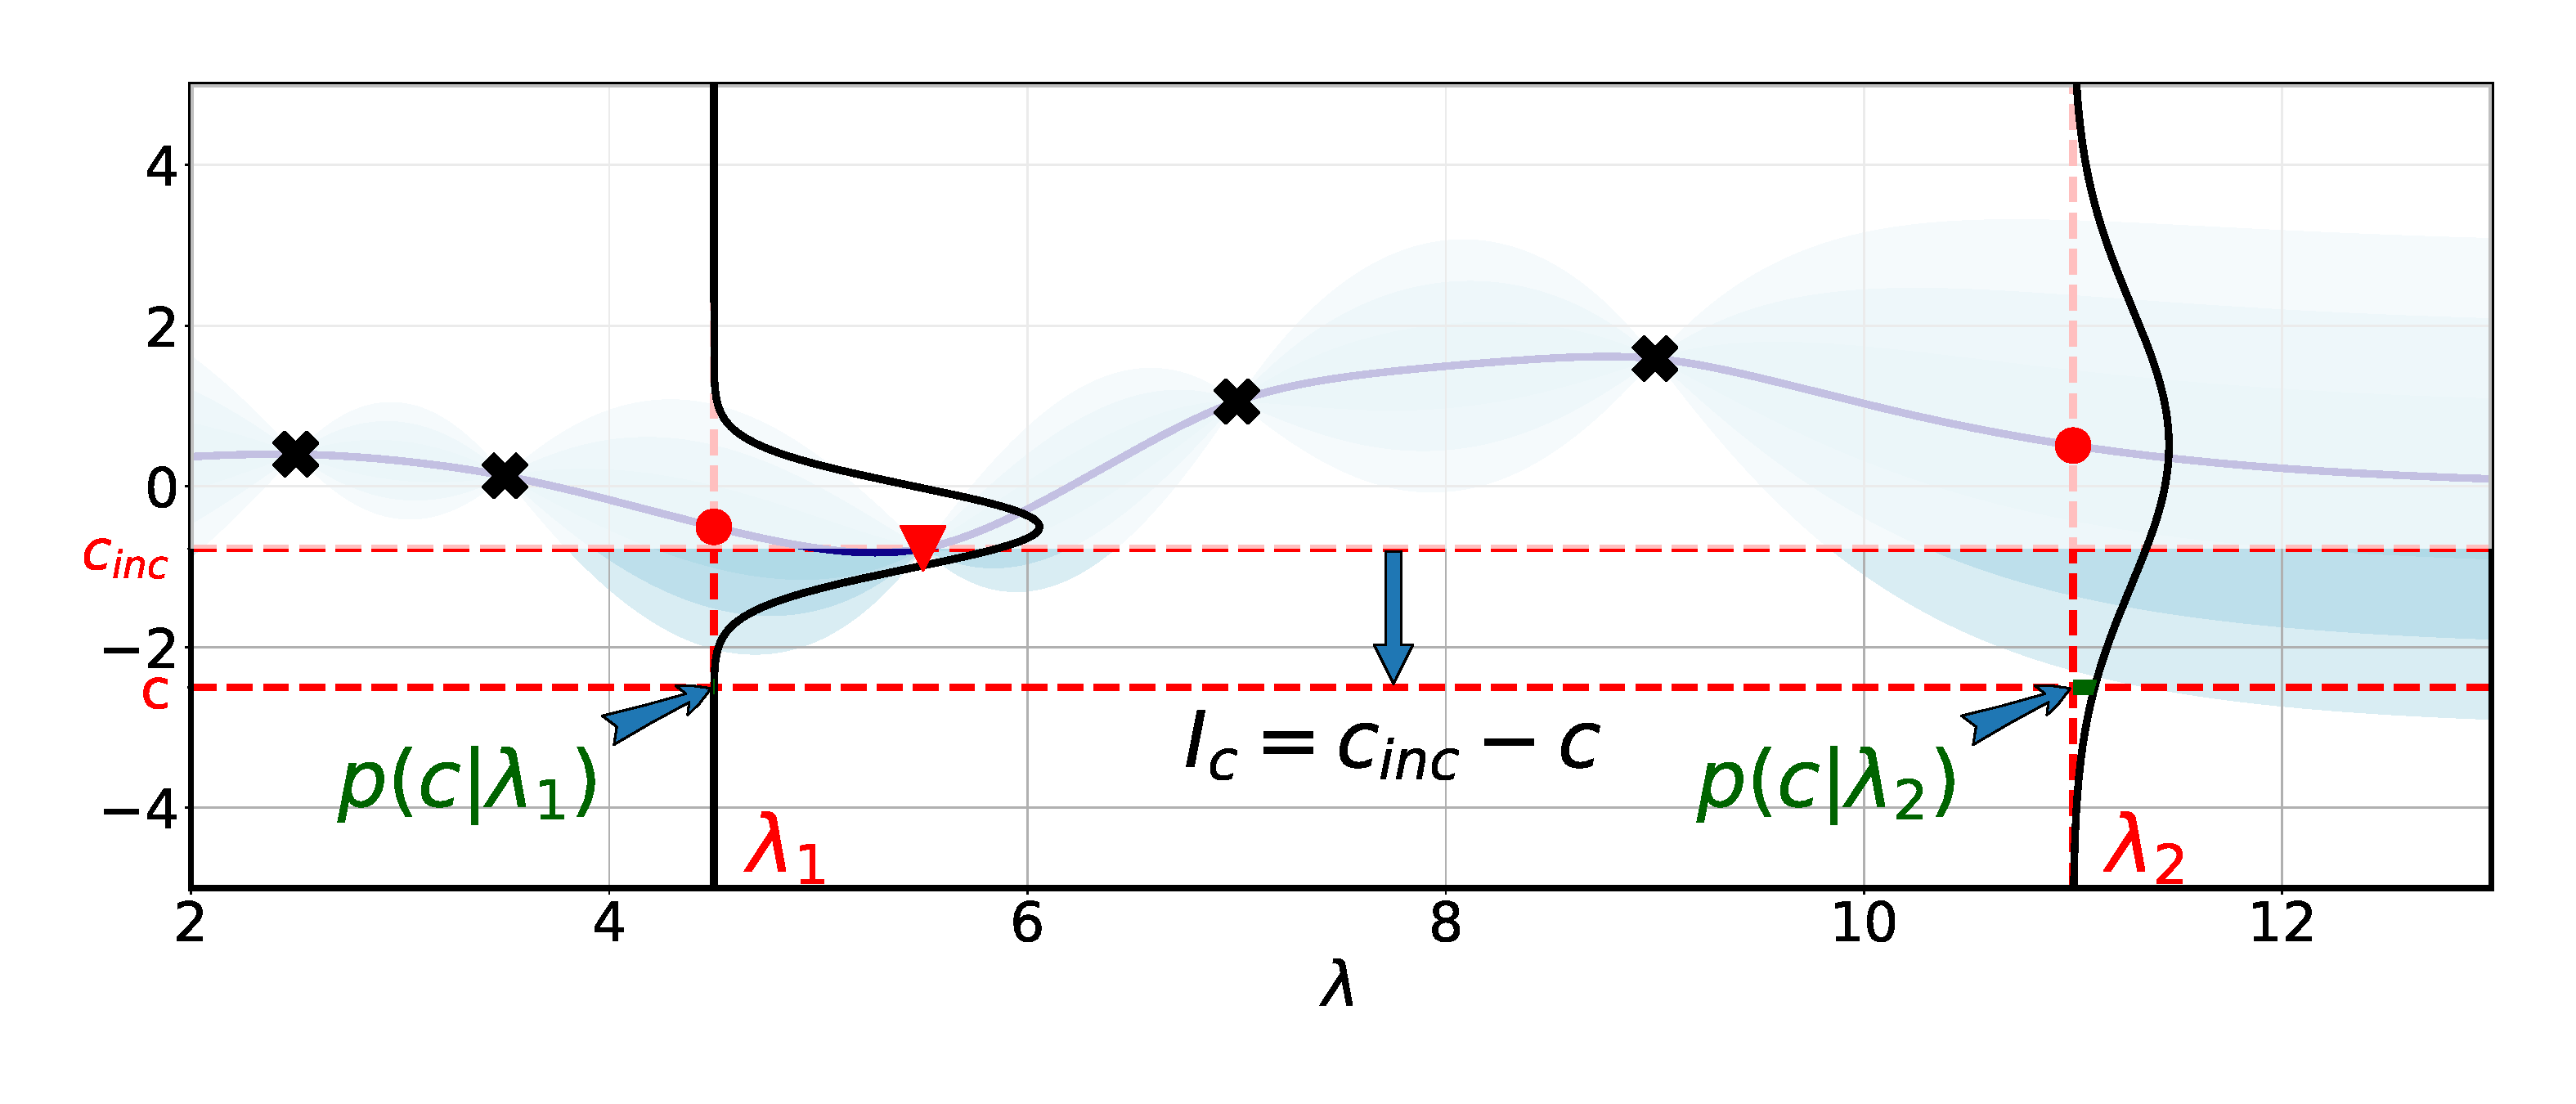
\includegraphics[width=\linewidth, height=0.7\textheight, keepaspectratio=true]{images/acq_func_images/ei/ei_7.pdf}};
    \node<.> [below=0.01\belowcaptionskip of img7, align=center]{Now consider the likelihood of a larger improvement.};
    
    \node<+> (img8) {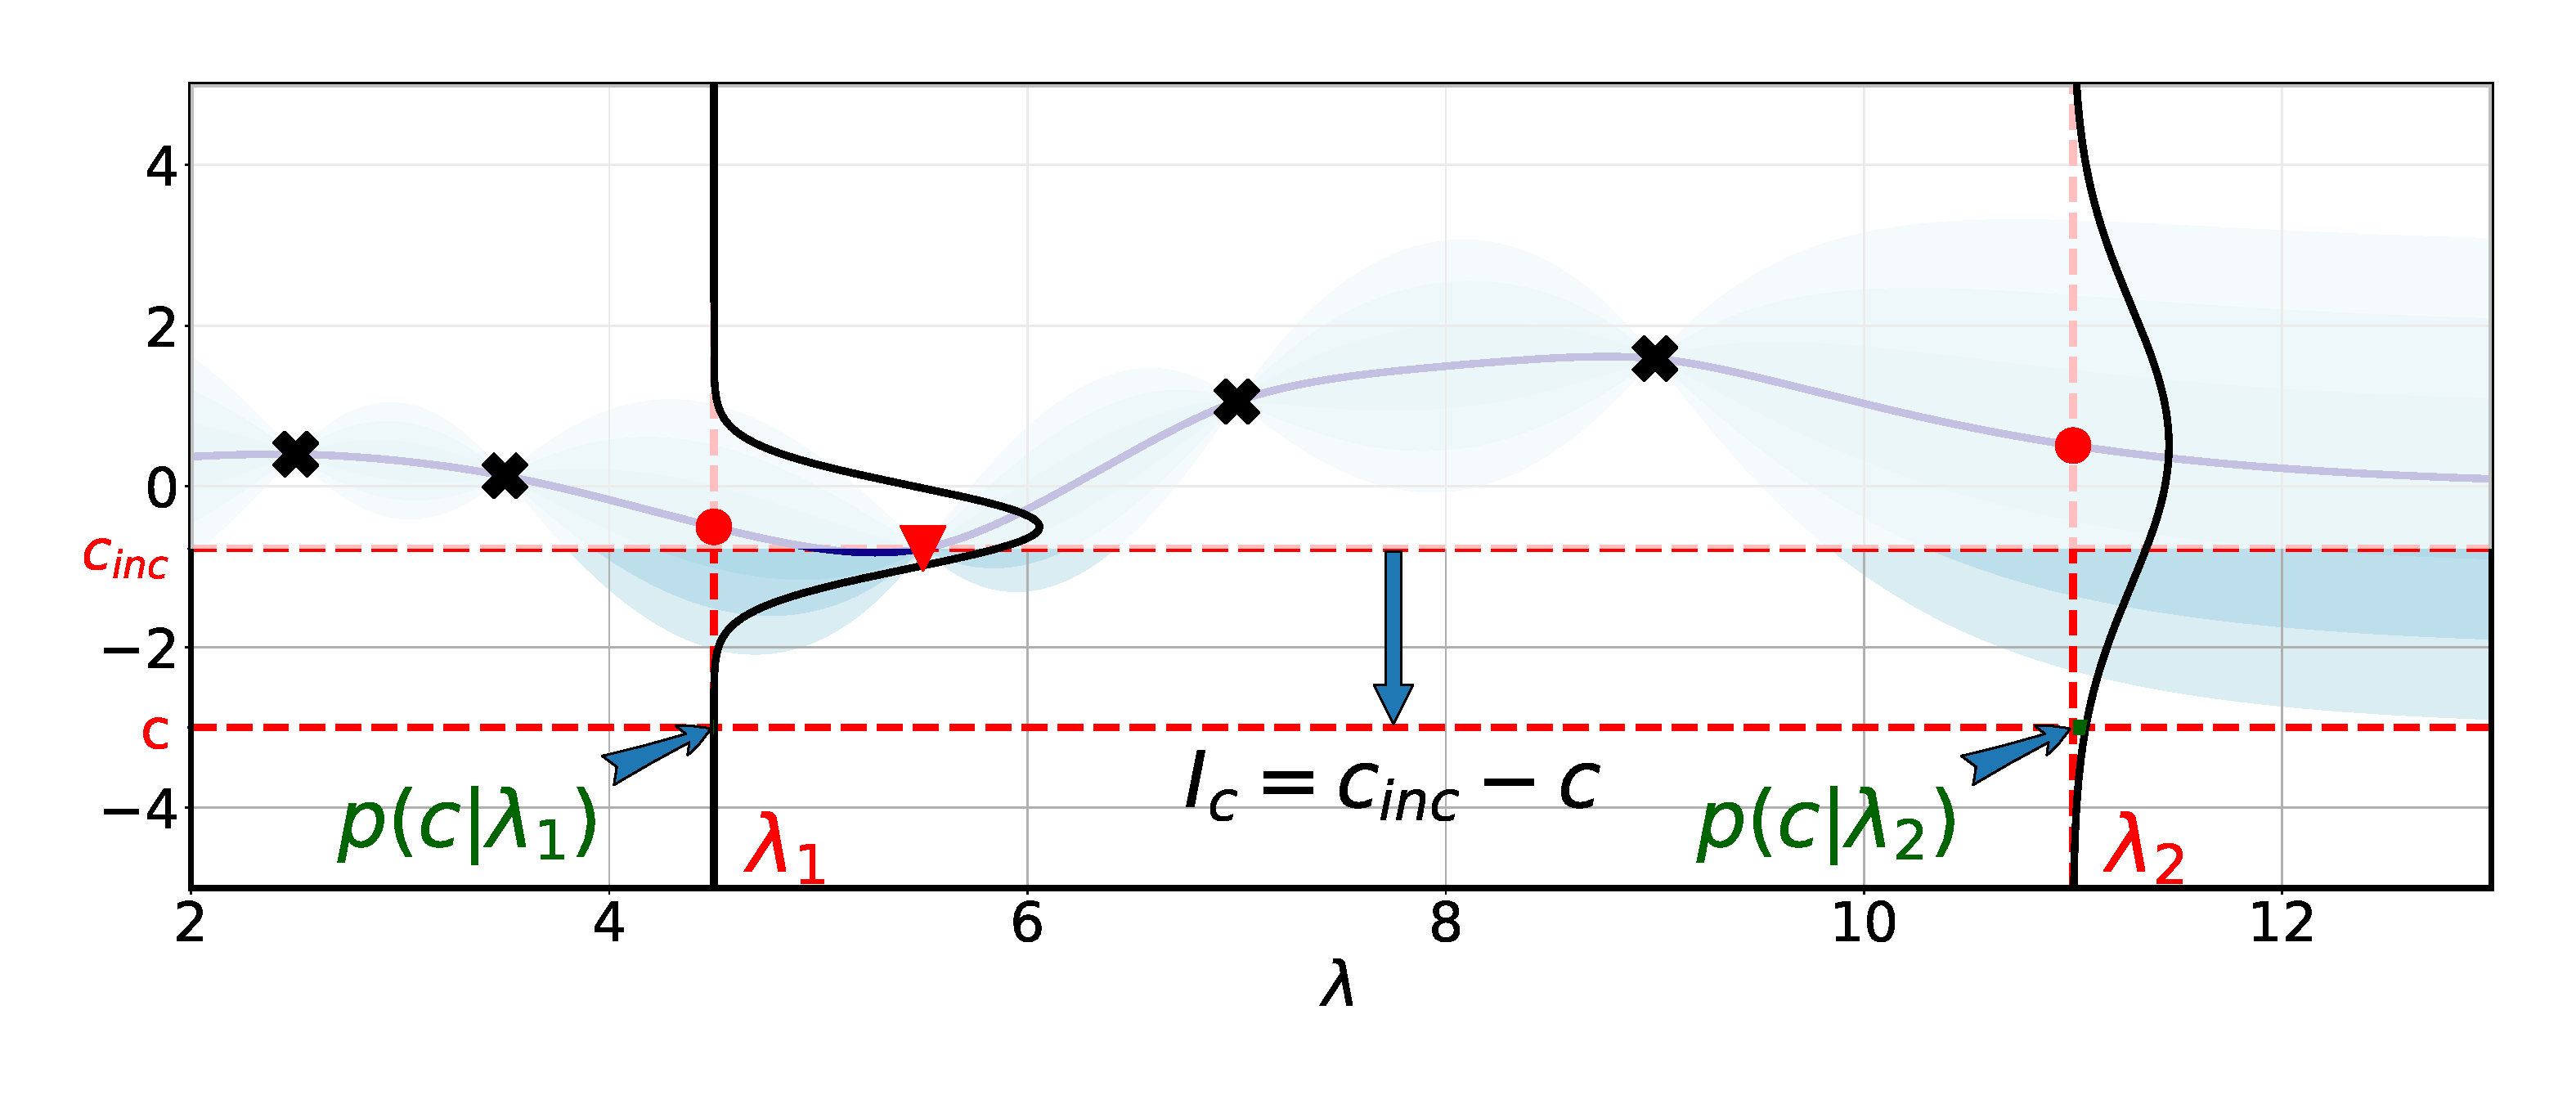
\includegraphics[width=\linewidth, height=0.7\textheight, keepaspectratio=true]{images/acq_func_images/ei/ei_8.pdf}};
    \node<.> [below=-0.01\belowcaptionskip of img8, align=center]{Larger improvements are more likely in areas of high uncertainty.\\ To compute $\E[I(\conf)]$, intuitively, we sum $p(\cost \mid \conf) \times I_\cost$ over all possibles values of $\cost$.
    %\\We can thus use $\surro(\conf) = \normaldist( \mean(\conf), \variance(\conf))$ to calculate $\E[\iter{I}(\conf)]$.
    };

  \end{tikzpicture}
% \end{figure}

\end{frame}
%-----------------------------------------------------------------------
\begin{frame}[c]{Expected Improvement (EI): Formal Definition}
%\framesubtitle{Expected Improvement - Choosing a candidate}
    \begin{itemize}\abovedisplayskip=0em\belowdisplayskip=-0.75em
        \item We define the one-step positive \alert{improvement over the current incumbent} as
        \smallskip
        \[
            \alert{\iter{I}(\conf) = \max(0, \cost_{inc} - \cost(\conf))}
        \]
%        \comment{This is probably a great time to point out, once again, that because I is defined in terms of the actual cost function, we cannot directly compute it.}
        \smallskip
        \item Expected Improvement is then defined as \alert{\[\iter{\acq}_{EI}(\conf) = \E[\iter{I}(\conf)] = \int_{-\infty}^{\infty} \iter{p}(\cost \mid \conf) \times \iter[\bocount]{I}(\conf)\;\; d\cost.\]}
        \pause
        \smallskip
        \item Since the posterior distribution of $\surro(\conf)$ is a Gaussian, EI can be computed in closed form (see exercise):
        
%        \comment{Maybe emphasize that this is actually how and where the dependence on the actual cost function is replaced with a dependence on the surrogate.}
        \begin{align*}
            \alert{\iter{\acq}_{EI}(\conf)} &\alert{=} 
            \begin{cases}
                \alert{\iter{\stddev}(\conf)[Z\cdf(Z) + \pdf(Z)]}, & \text{if }\iter{\stddev}(\conf) > 0 \\
                0 & \text{if }\iter{\stddev}(\conf) = 0,
            \end{cases}\\
            \text{where }Z &=\dfrac{\cost_{inc} - \iter{\mean}(\conf) - \xi}{\iter{\stddev}(\conf)}
            \text{ and } \xi \text{ is an optional exploration parameter.}
        \end{align*}
%            \comment{I believe I needed to switch the signs of $\cost(\cdot)$ and $\mean(\cdot)$ as compared to the reference paper in order to accommodate for our convention of minimization/maximization. Please cross-check!}
    \pause
    \bigskip
    \[\boxed{\text{Choose}\;\;\bonextsample \in \argmax_{\conf\in\pcs}(\iter{\acq}_{EI}(\conf))}
    \]
    \end{itemize}
\end{frame}
%-----------------------------------------------------------------------
%\begin{frame}[c]{Computationally Cheap Acquisition Functions - EI}
%\framesubtitle{Expected Improvement - Choosing a candidate}
%\comment{Verify if formulae agree with minimizing the surrogate.}
%    \begin{itemize}\abovedisplayskip=0pt\belowdisplayskip=-0.5em
%        \item[] We first define one-step improvement over the current incumbent, as
%        \smallskip
%        \[
%            \iter{I}(\conf) = \max(0, \cost(\incumbent[\bocount-1]) - \cost(\conf)), \quad\incumbent[\bocount-1]\in\argmin_{\conf'\in\iter[\bocount-1]{\dataset}}\obs[\conf']\in\iter[\bocount-1]{\dataset}
%        \]
%        \comment{This is probably a great time to point out, once again, that because I is defined in terms of the actual cost function, we cannot directly compute it.}
%        \pause
%        \medskip
%        \item[] Expected Improvement is then defined as
%        \begin{align*}
%            \iter{\acq}_{EI}(\conf) &= \E[\iter{I}(\conf)]\\
%            &= \int_{\iter{I}=0}^{\iter{I}=\infty}\iter{I} P(\iter{I})d\iter{I}
%        \end{align*}
%        \pause
%        \medskip
%        \item[]Since the posterior distribution of the surrogate is a Gaussian, it can be shown that the distribution on $\iter{I}(\conf)$ is also a Gaussian, defined as
%        \[
%            P(\iter{I}) =
%                \dfrac{1}{\sqrt{2\pi}\iter{\stddev}(\conf)}\exp{\left[-\dfrac{{(\cost(\incumbent[\bocount-1])-\iter{\mean}(\conf)-\iter{I})}^2}{2\iter{\left(\variance\right)}(\conf)}
%            \right]}
%        \]
%        \comment{Maybe emphasize that this is actually how and where the dependence on the actual cost function is replaced with a dependence on the surrogate.}
%    \end{itemize}
%\end{frame}
%-----------------------------------------------------------------------
% \begin{frame}[c]{Computationally Cheap Acquisition Functions - EI}
% \framesubtitle{Expected Improvement - Choosing a candidate}
%     \begin{align*}
%         \action<+->{\iter{\acq}_{EI}(\conf) &= \int_{\iter{I}=0}^{\iter{I}=\infty}\iter{I} \dfrac{1}{\sqrt{2\pi}\iter{\stddev}(\conf)}\exp{-\dfrac{{(\cost(\incumbent[\bocount-1])-\iter{\mean}(\conf)-\iter{I})}^2}{2\iter{\left(\variance\right)}(\conf)}}d\iter{I}\\}
%         \action<+->{&= 
%             \begin{cases}
%                 (\cost(\incumbent) - \iter{\mean}(\conf) - \xi)\cdf(Z) + \iter{\stddev}(\conf) \pdf(Z), & \text{if }\iter{\stddev}(\conf) > 0 \\
%                 0 & \text{if }\iter{\stddev}(\conf) = 0
%             \end{cases}\\}
%         \action<+->{\intertext{where }Z} \action<.->{&=\dfrac{\cost(\incumbent) - \iter{\mean}(\conf) - \xi}{\iter{\stddev}(\conf)}}
%     \action<+->{\Aboxed{\bonextsample \in \argmax_{\conf\in\pcs}(\iter{\acq}_{EI}(\conf))}}
%     \end{align*}
% %    \comment{Source: Tutorial by Brochu et al.: https://arxiv.org/pdf/1012.2599.pdf }
% \end{frame}
%-----------------------------------------------------------------------
%\begin{frame}[c]{Computationally Cheap Acquisition Functions - EI}
%\framesubtitle{Expected Improvement - Choosing a candidate}
%    \begin{align*}
%        \action<+->{\iter{\acq}_{EI}(\conf) &= \int_{\iter{I}=0}^{\iter{I}=\infty}\iter{I} \dfrac{1}{\sqrt{2\pi}\iter{\stddev}(\conf)}\exp{-\dfrac{{(\cost(\incumbent[\bocount-1])-\iter{\mean}(\conf)-\iter{I})}^2}{2\iter{\left(\variance\right)}(\conf)}}d\iter{I}\\}
%        \action<+->{&= 
%            \begin{cases}
%                \iter{\stddev}(\conf)[Z\cdf(Z) + \pdf(Z)], & \text{if }\iter{\stddev}(\conf) > 0 \\
%                0 & \text{if }\iter{\stddev}(\conf) = 0
%            \end{cases}\\
%            \intertext{where }Z &=\dfrac{\cost(\incumbent[\bocount-1]) - \iter{\mean}(\conf) - \xi}{\iter{\stddev}(\conf)}}
%            \comment{I believe I needed to switch the signs of $\cost(\cdot)$ and $\mean(\cdot)$ as compared to the reference paper in order to accommodate for our convention of minimization/maximization. Please cross-check!}
%    \action<+->{\Aboxed{\text{Choose}\,\bonextsample \in \argmax_{\conf\in\pcs}(\iter{\acq}_{EI}(\conf))}}
%    \end{align*}
%    \comment{Source: Tutorial by Brochu et al.: https://arxiv.org/pdf/1012.2599.pdf }
%\end{frame}
%-----------------------------------------------------------------------
\begin{frame}[t]{Lower/Upper Confidence Bounds (LCB/UCB): Concept}

% \begin{figure}
  \centering
  \begin{tikzpicture}
    \node<+> (img1) {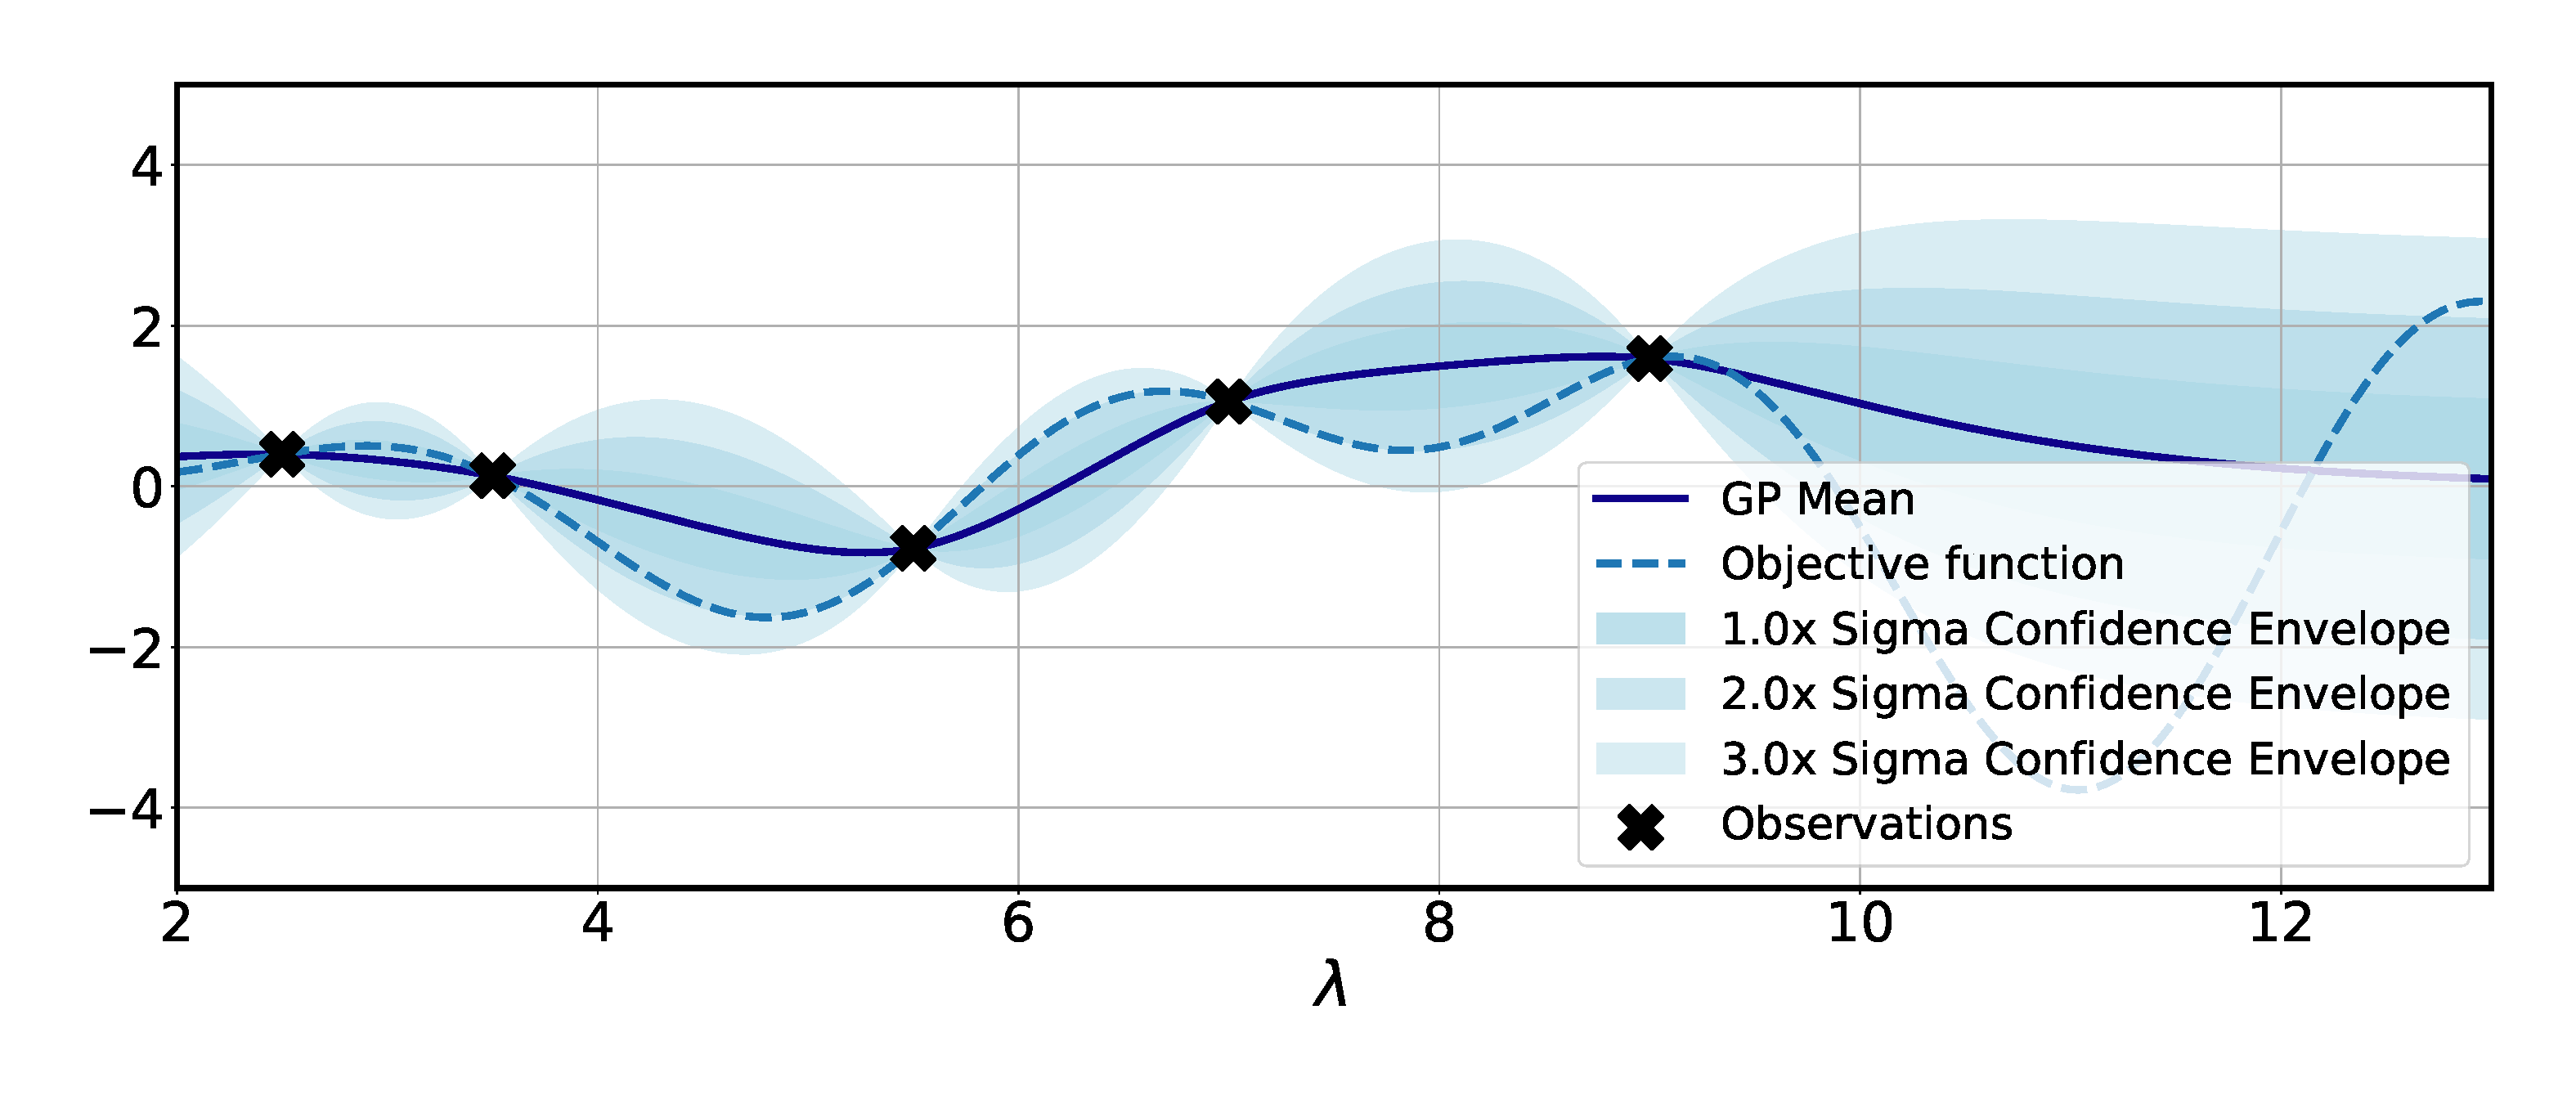
\includegraphics[width=\linewidth, height=0.7\textheight, keepaspectratio=true]{images/acq_func_images/lcb/lcb_1.pdf}};
    \node<.> [below=0.01\belowcaptionskip of img1, align=center]{Given the surrogate fit at iteration $\bocount$};
    %fit on dataset $\iter[\bocount-1]{\dataset}$};
    \node<+> (img2) {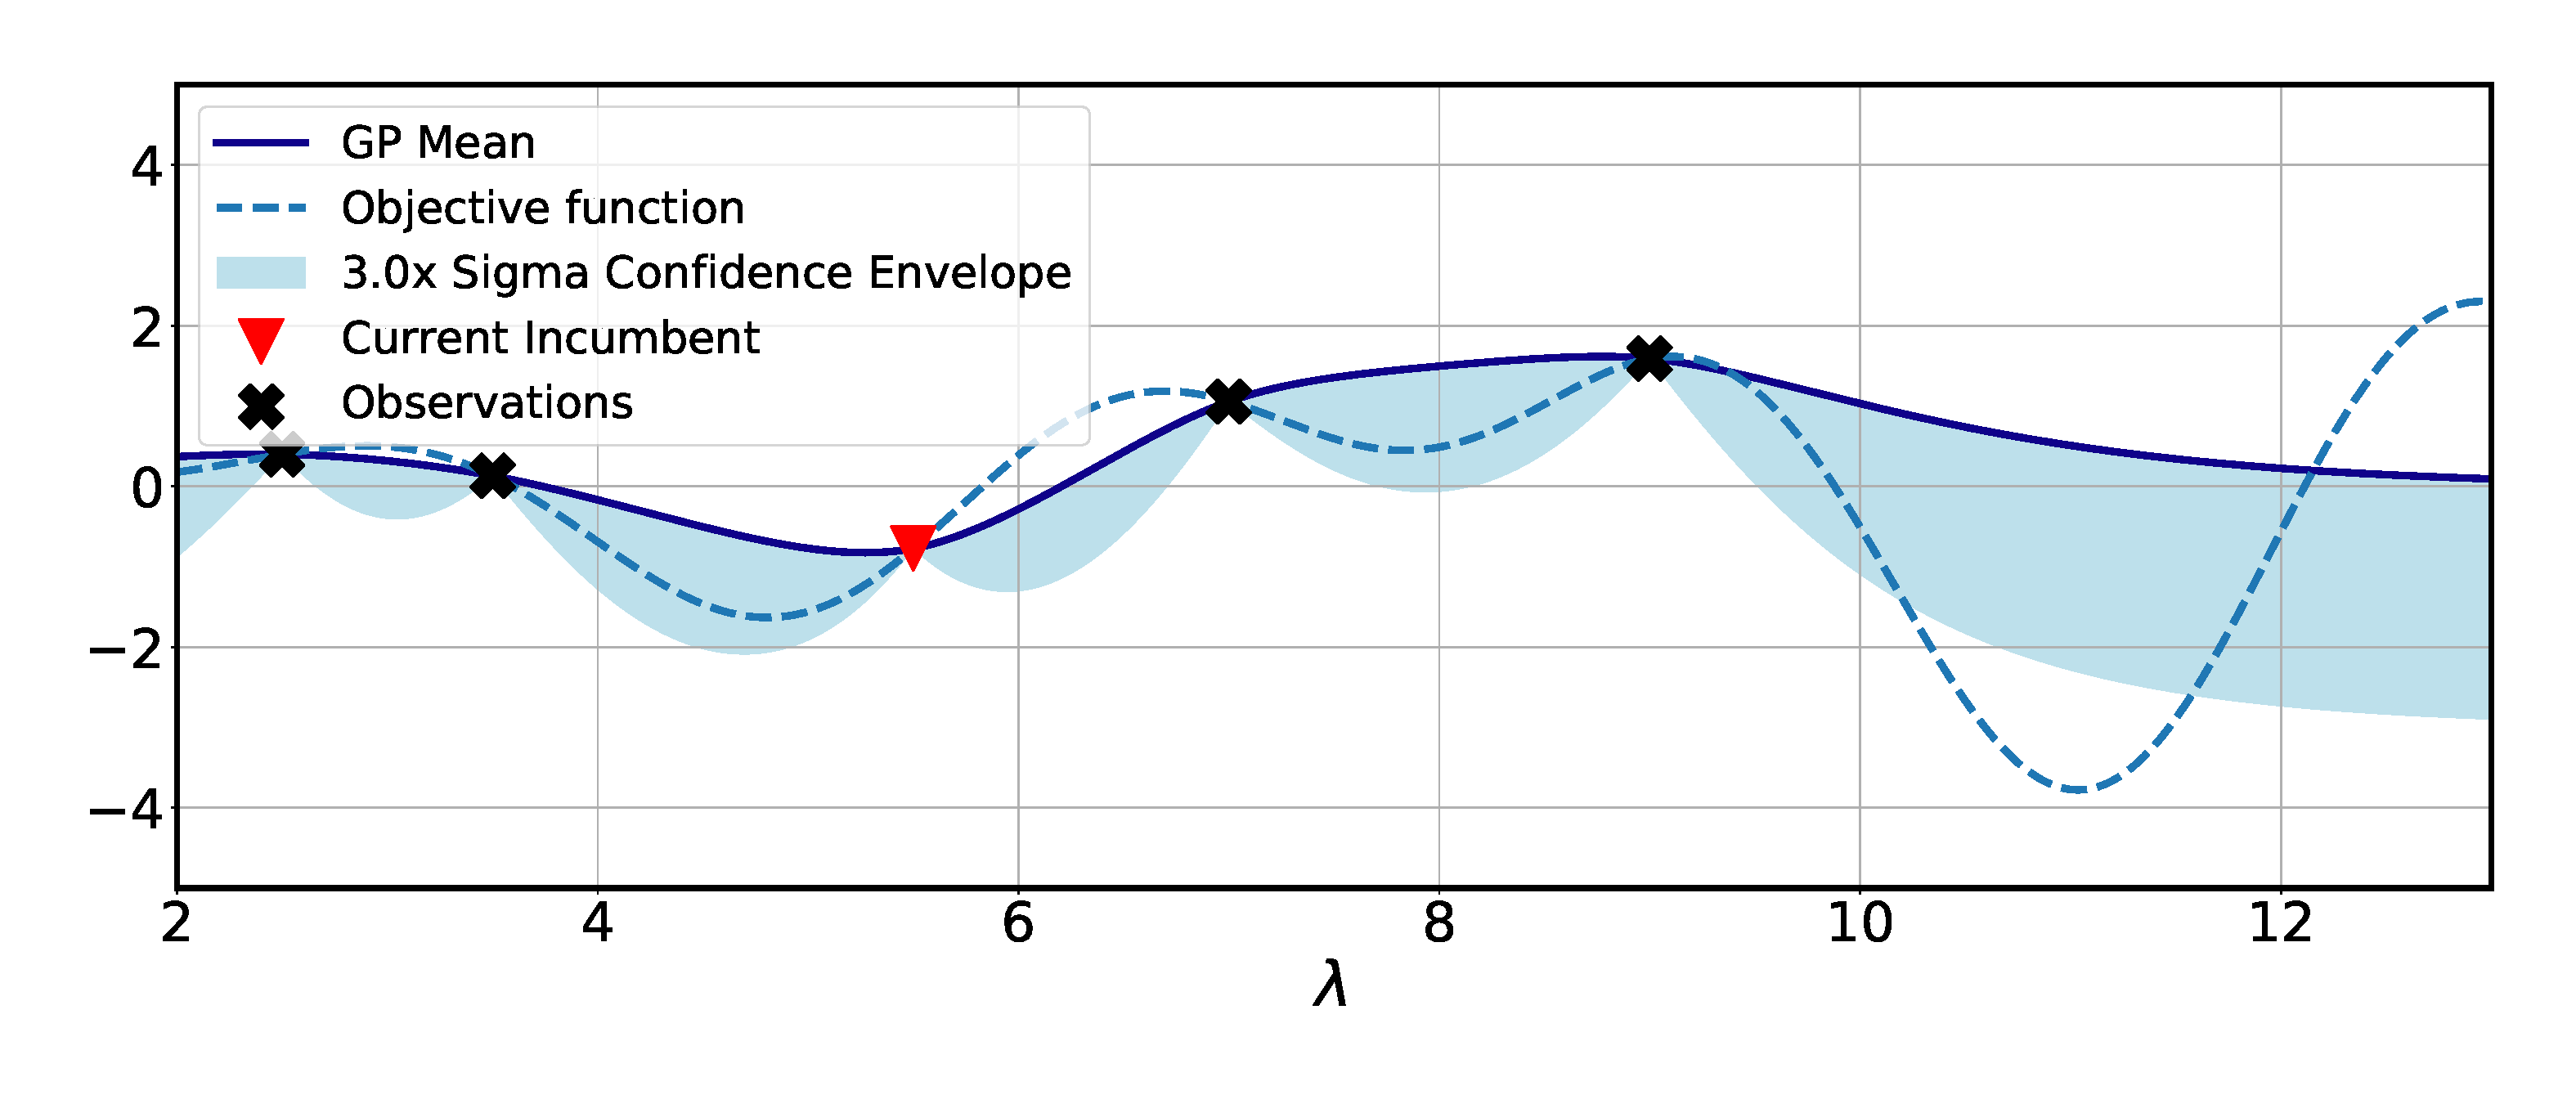
\includegraphics[width=\linewidth, height=0.7\textheight, keepaspectratio=true]{images/acq_func_images/lcb/lcb_2.pdf}};
    \node<.> [below=0.01\belowcaptionskip of img2, align=center]{Lower Confidence Bound, $\mean(\conf)-\alpha\stddev(\conf)$ (here, for $\alpha=3$)};
  \end{tikzpicture}
% \end{figure}

\end{frame}
%-----------------------------------------------------------------------
\begin{frame}[c]{Lower/Upper Confidence Bounds (LCB/UCB): Formal Definition}
\begin{itemize}
    \item We define the \alert{Lower Confidence Bound} as
    \[\alert{\iter{\acq}_{LCB}(\conf) = \iter{\mean}(\conf) - \alpha\iter{\stddev}(\conf)},\quad\alpha\geq0\]

\bigskip
    \item One can schedule $\alpha$ (e.g., increase it over time \lit{\href{https://arxiv.org/pdf/0912.3995.pdf}{Srinivas et al. 2009}})

\[
    \boxed{\text{Choose}\;\;\bonextsample \in \argmax_{\conf\in\pcs}\left(\alert{-} \iter{\acq}_{LCB}(\conf)\right)}
\]

\end{itemize}
    \bigskip
    \pause
    
    \myit{
        \item Note: when one aims to \alert{maximize} the objective function, one would use \alert{UCB} instead
        \myit{
            \item $\iter{\acq}_{UCB}(\conf)) = \iter{\mean}(\conf) + \alpha\iter{\stddev}(\conf)$ 
            \item For UCB, one would choose $\bonextsample \in \argmax_{\conf\in\pcs}( \iter{\acq}_{UCB}(\conf))$ 
        }
    }
%    \item It has been shown that using the acquisition function
%    \[\iter{\acq}_{GP-LCB}(\conf) = \iter{\mean}(\conf) - \sqrt{\nu\tau_t}\iter{\stddev}(\conf), \quad\nu>0,\] asymptotically results in zero cumulative regret with the appropriate choice of parameters $\tau$ and $\nu$ \lit{\href{https://arxiv.org/pdf/0912.3995.pdf}{Srinivas et al. 2009}}.}
%    \comment{Trying to further explain the difference between LCB and GP-LCB's parameters would've overwhelmed the intuitiveness of the slide. Instead, a quick verbal note on the difference and pointing out the reference paper by Srinivas et al. for further reading should suffice.}
    %\comment{Source: Tutorial by Brochu et al.: https://arxiv.org/pdf/1012.2599.pdf }
\end{frame}
%-----------------------------------------------------------------------
\begin{frame}[t]{Thompson Sampling (TS): Concept}

% \begin{figure}
  \centering
  \begin{tikzpicture}
    \node<+> (img1) {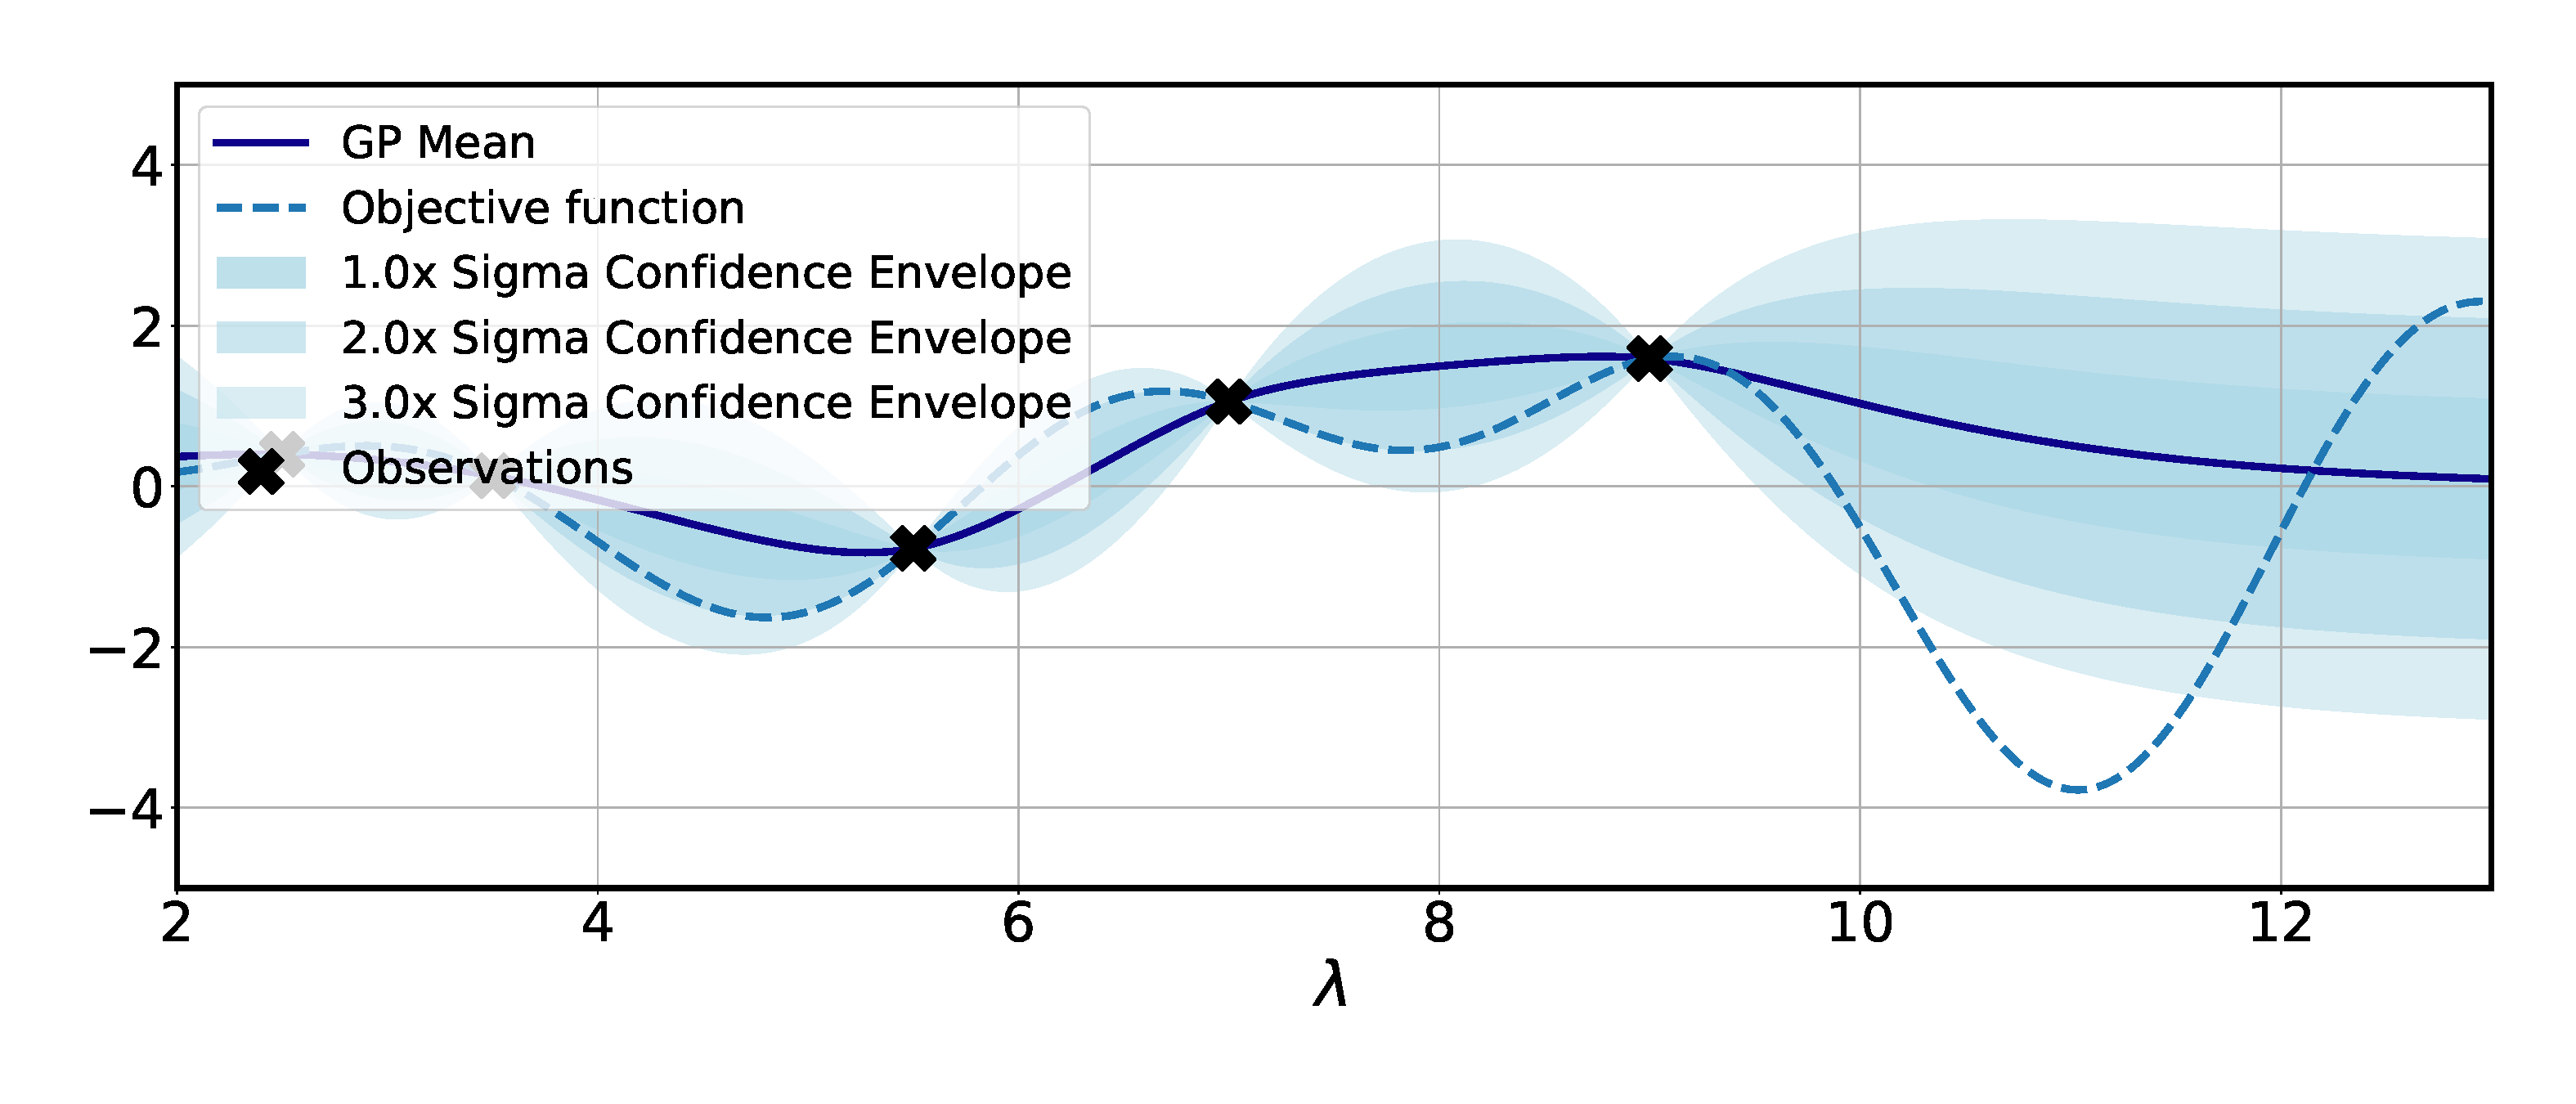
\includegraphics[width=\linewidth, height=0.7\textheight, keepaspectratio=true]{images/acq_func_images/ts/ts_1.pdf}};
    \node<.> [below=0.01\belowcaptionskip of img1, align=center]{Given the surrogate at iteration $\bocount$ fit on dataset $\iter[\bocount-1]{\dataset}$};
    \node<+> (img2) {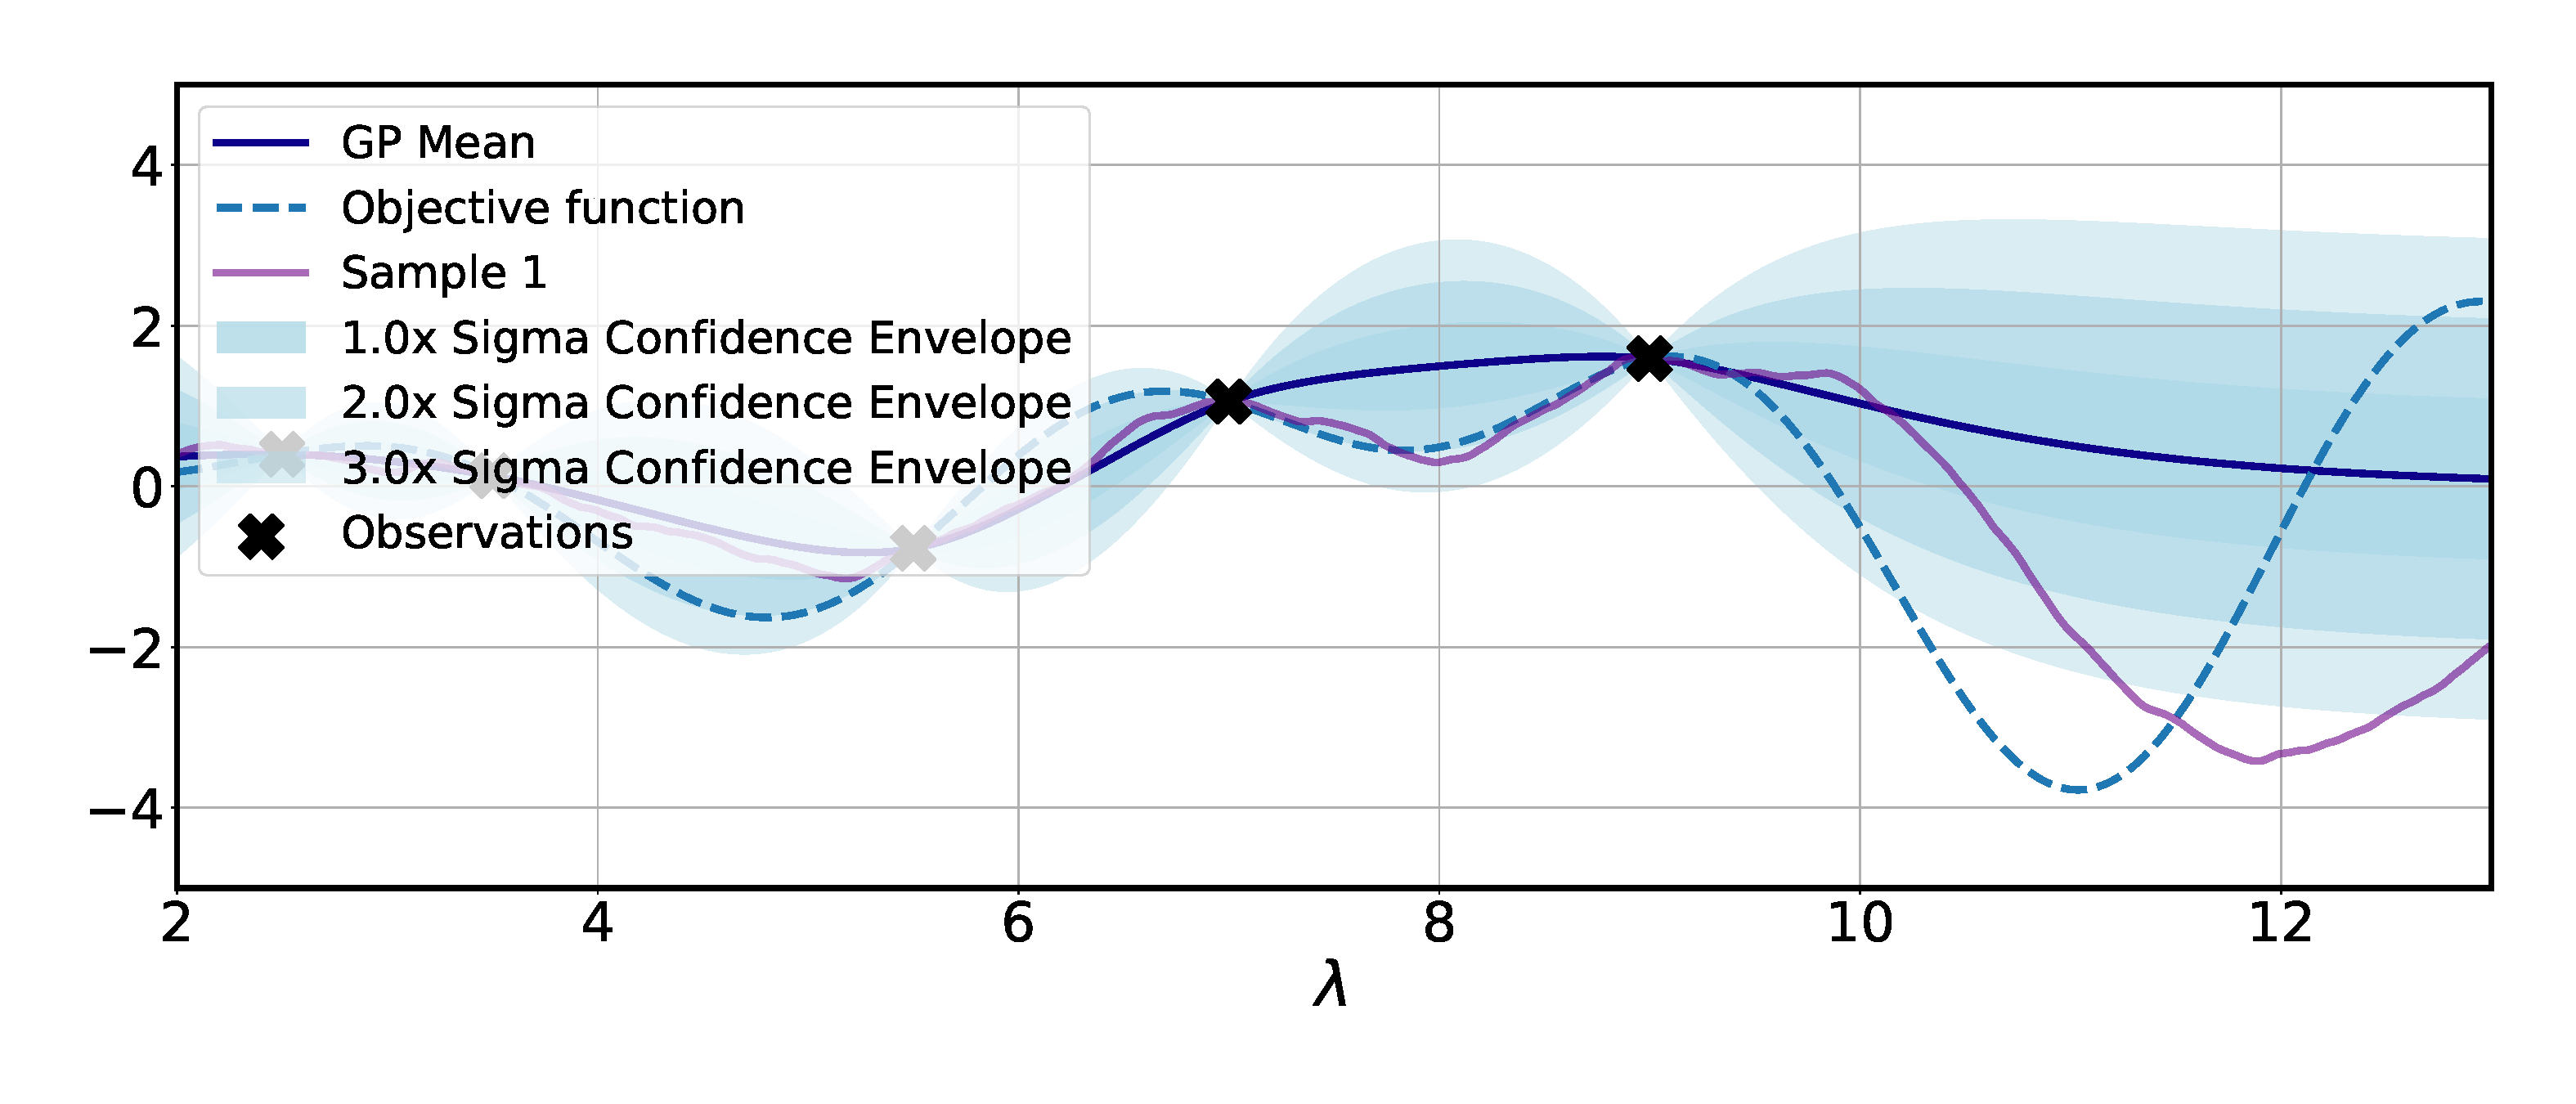
\includegraphics[width=\linewidth, height=0.7\textheight, keepaspectratio=true]{images/acq_func_images/ts/ts_2.pdf}};
    \node<.> [below=0.01\belowcaptionskip of img2, align=center]{Draw a sample $g$ from the predictive surrogate model};
    \node<+> (img3) {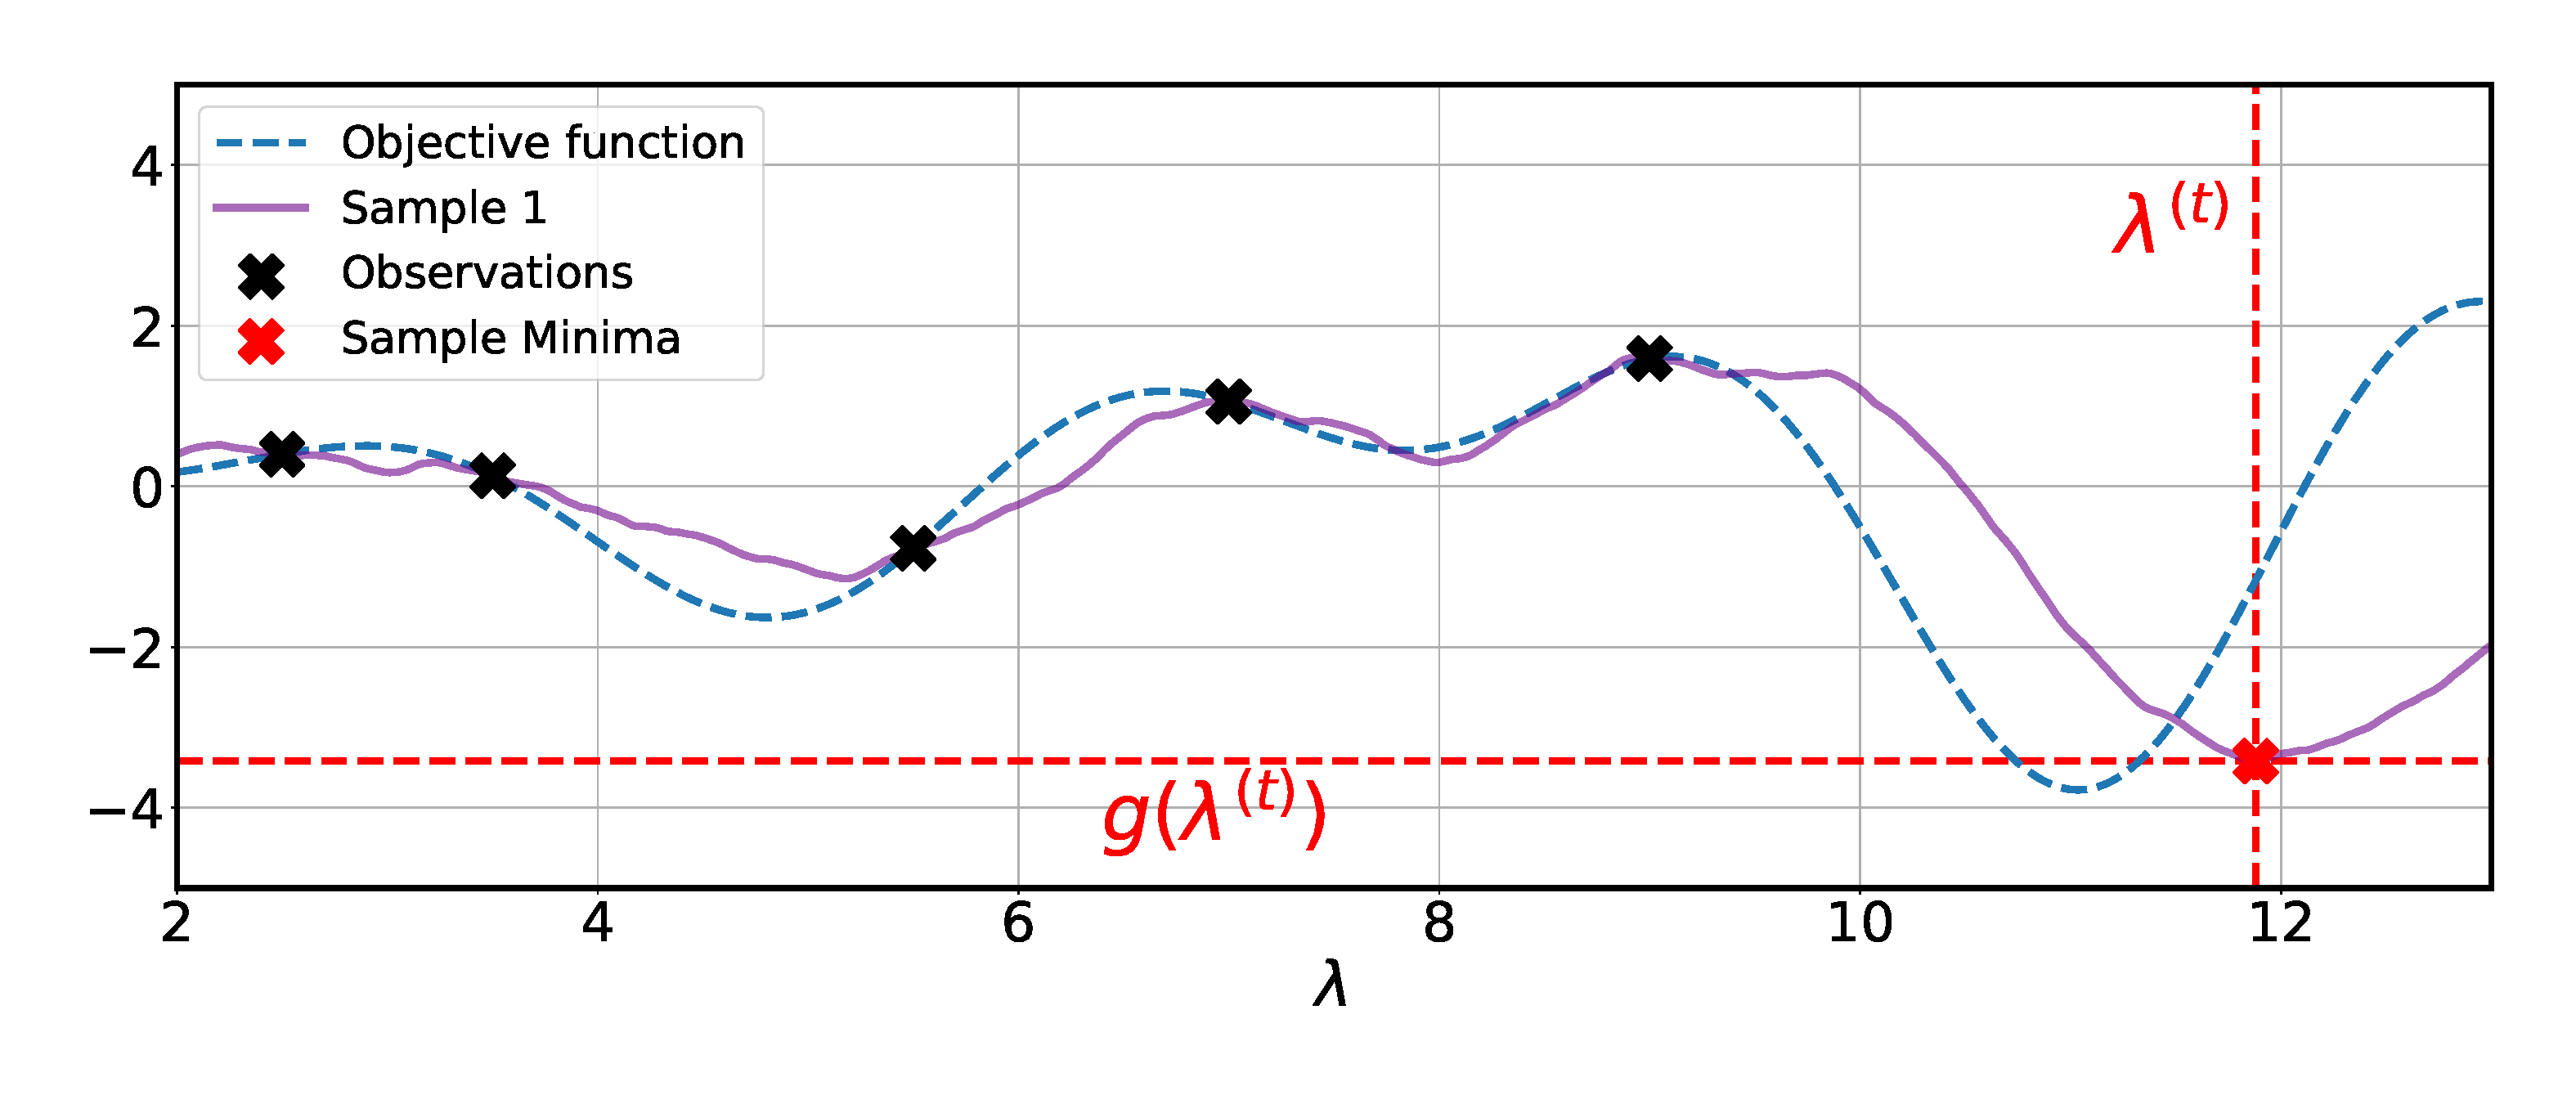
\includegraphics[width=\linewidth, height=0.7\textheight, keepaspectratio=true]{images/acq_func_images/ts/ts_3.pdf}};
    \node<.> [below=0.01\belowcaptionskip of img3, align=center]{Then choose the minimum of this sample to evaluate at next};
  \end{tikzpicture}
% \end{figure}

\end{frame}
%-----------------------------------------------------------------------
% \begin{frame}[c]{Computationally Cheap Acquisition Functions - TS}
% \framesubtitle{Thompson Sampling - Gist}
% 
% \begin{itemize}
%     \item Draw a sample $g$ from the GP $\iter{\gp}$.
%     \item Choose $\bonextsample=\argmin_{\conf\in\pcs}(g(\conf))$
% \end{itemize}
% \end{frame}
%-----------------------------------------------------------------------
\begin{frame}[c]{Thompson Sampling (TS): Pseudocode}

\begin{center}
\begin{minipage}{0.75\textwidth}
\comment{Fix algorithm numbering}
\begin{algorithm}[H]
    %\DontPrintSemicolon
    \LinesNumbered
%    \SetAlgoLined
    \setcounter{AlgoLine}{0}
    \SetKwInOut{Require}{Require}
    \SetKwInOut{Result}{Result}
    
    \Require{Search space $\pcs$, 
    		cost function $\cost$, 
    		surrogate model $\surro$,
    		maximal number of function evaluations $\bobudget$}
\Result{Best observed configuration $\finconf$ according to $\iter[\bobudget]{\dataset}$ or $\gp$}    
	Initialize data $\iter[0]{\dataset}$ with initial observations\;% \leftarrow \varnothing$\; 
    
    \For{$\bocount=1$ \KwTo $\bobudget$}{
    
		Fit predictive model $\iter[\bocount]{\surro}$ on $\iter[\bocount-1]{\dataset}$\;
    
        \textcolor{blue}{Sample a function from the surrogate: $g\sim\iter{\surro}$}\;
    
        \textcolor{blue}{Select next query point: $\bonextsample \in \argmin_{\conf\in\pcs}g(\conf)$}\;
    
        Query $\bonextobs$\;

    	Update data: $\iter[\bocount]{\dataset} \leftarrow \iter[\bocount-1]{\dataset} \cup \{\langle \bonextsample, \bonextobs \rangle \}$\;
        }
    \caption*{Bayesian Optimization using Thompson Sampling}
\end{algorithm}
\end{minipage}
\end{center}
%\comment{Source: Paper, Kandasamy et al, http://proceedings.mlr.press/v84/kandasamy18a/kandasamy18a.pdf}
\end{frame}
%-----------------------------------------------------------------------
\begin{frame}[c]{Questions to Answer for Yourself / Discuss with Friends}

\begin{itemize}
%PI
    \item \alert{Discussion.} How would you set the exploration parameter $\xi$ for PI if you want to avoid too incremental improvements?
\medskip
%EI
    \item \alert{Derivation.} Derive the closed form solution of expected improvement.
\medskip
    \item \alert{Discussion.} In which situations would EI perform substantially differently than PI?
%LCB
%TS
\end{itemize}

\end{frame}